\documentclass[12pt, a4paper, oneside]{book}
\usepackage{tfg}


\newtheorem{theorem}{Theorem}

\DeclareMathOperator{\normal}{Normal}
\DeclareMathOperator{\id}{id}
\DeclareMathOperator{\attentionop}{Attention}
\DeclareMathOperator{\softmax}{softmax}
\DeclareMathOperator{\argmax}{arg max}
\renewcommand\tabularxcolumn[1]{m{#1}}% for vertical centering text in X column

\newcommand{\real}[1]{\mathbb{R}^{#1}}
\newcommand{\kaggle}{https://www.kaggle.com/competitions/diabetic-retinopathy-detection/overview}

\addbibresource{references.bib}
\usepackage{url}
\def\UrlBreaks{\do\/\do—}

\begin{document}
    \newpage
\thispagestyle{empty}

\begin{center}
    \rule{7cm}{1pt} \\
    \vspace*{0.2cm}
    \Large{Diabetic retinopathy diagnosis using deep learning} \\
    \vspace*{0.2cm}
    \hspace*{-0.8cm}\mbox{\large{Diagnóstico de la retinopatía diabética usando aprendizaje profundo}} \\
    \vspace*{0.2cm}
    \rule{7cm}{1pt} \\
    \vspace*{1cm} 
    \includegraphics[height=2in]{figures/escudo.png} \\
    \vspace{0.75cm}
    \Large{Trabajo de fin de grado en Ingeniería Informática} \\
    \Large{Curso 2022-2023} \\
    \vspace{0.75cm}
    \large{\textbf{Autores}} \\
    \large{Luis Ariza López} \\
    \large{Álvaro Sanz Ramos} \\ 
    \vspace{0.25cm}
    \large{\textbf{Director}} \\
    \large{Prof. Antonio Alejandro Sánchez Ruiz-Granados} \\

    \vspace{0.75cm}
    Doble grado en Ingeniería Informática — Matemáticas \\
    Facultad de informática \\
    Universidad Complutense de Madrid \\
    \vspace{1cm}
\end{center}

    \newpage
    % +--------------------------------------------------------------------+
% | Copyright Page
% +--------------------------------------------------------------------+

\newpage

\thispagestyle{empty}

\section*{Abstract}
Diabetic retinopathy (DR) is one of the main complications of diabetes and the leading cause of new cases of blindness. Early detection is fundamental for a good prognosis, but diagnosis is a hard, expensive and time-consuming process. The need of automating methods for DR grading was recognized time ago, but most approaches in literature require vast computational power and have not been designed with interpretability in mind.

We show that a model based in a convolutional neural network can achieve excellent performance at DR grading, comparing favorably to much larger models and achieving state-of-the-art results. Using transfer learning, we reduce to the minimum the computational requirements: the model can be trained in a few hours on domestic hardware.

We use the hidden representation learned by the model to identify images diagnostically similar to a given one and explore the possibility of using this model in a clinical setting in a series of test carried on collaboration with a professional ophthalmologist. According to the criterion of the professional, the tool correctly identifies similar images and is a helpful assistance during diagnosis.

Furthermore, we implement several interpretability tools to understand how the model makes predictions, address important concerns for clinical application (as calibration) and compare our approach to an alternative one using Vision Transformers under strict computational requirements.

\section*{Keywords}
Deep learning, convolutional neural networks, classification, computer vision, diabetic retinopathy, Vision Transformers, transfer learning, model calibration, model interpretability, medical image analysis.



    \newpage
    % +--------------------------------------------------------------------+
% | Copyright Page
% +--------------------------------------------------------------------+

\newpage

\thispagestyle{empty}

\section*{Resumen}
La retinopatía diabética es una de las principales complicaciones de la diabetes y la principal causa de nuevos casos de ceguera. Detectar esta enfermedad en sus primeras etapas es clave para un buen pronóstico, pero el diagnóstico es un proceso difícil, caro y que requiere tiempo. Para solventar estos inconvenientes se han desarrollado métodos que automatizan el diagnóstico, pero la mayor parte de ellos requieren grandes recursos computacionales y no son interpretables.

En este trabajo se demuestra que un modelo basado en redes convolucionales puede diagnosticar con gran precisión la retinopatía diabética a partir de  retinografías. El modelo, entrenado en pocas horas utilizando aprendizaje transferido y con requisitos computacionales mínimos, obtiene resultados punteros, superiores a los de modelos mucho más complejos.

Como ejemplo de la aplicabilidad de este modelo, hemos utilizado la representación interna aprendida por la red neuronal para identificar imágenes con características diagnósticas similares a una imagen base. Una serie de pruebas con una oftalmóloga profesional, asientan la posibilidad de utilizar el modelo en la práctica clínica: la profesional consideró que la herramienta era capaz de identificar imágenes similares consistentemente y resultaba de ayuda para realizar el diagnóstico.

También implementamos diversas técnicas de interpretabilidad para comprender el funcionamiento del modelo y abordamos posibles obstáculos para el uso práctico del modelo (como la calibración). Complementariamente, realizamos una comparación entre nuestro modelo y una aproximación basada en Vision Transformers. 

\section*{Palabras clave}
Aprendizaje profundo, redes neuronales convolucionales, clasificación, visión artificial, retinopatía diabética, Vision Transformers, aprendizaje transferido, calibración del modelo, interpretabilidad, análisis de imágenes médicas.

    \newpage
    \input{acknowledgment.tex}
    \tableofcontents

    \newpage

    \pagenumbering{arabic}
    \setcounter{page}{1}

    \cleardoublepage

\chapter{Introduction}
\label{chapter1}
\section{Motivation}
Increased life expectancy and sedentary lifestyles have boosted the appearance of chronic lifestyle-associated diseases. This has repercussions both at patient-level, with a significant loss of life quality, and at greater levels, increasing the pressure over national health systems.

Diabetes, which already affects one in ten adults, is undoubtedly one of the more damaging and harder to control. 783 million of people are projected to live with diabetes by 2045 and the cost of treating the disease has more than triplicated in the last 15 years \cite{diabetesatlas}.

A common complication of diabetes is diabetic retinopathy (DR) (around 40\% to 45\% of patients with diabetes have some stage of the disease\cite{drPatients}), caused by the vascular damages provoked by a persistently high blood sugar level. DR is already the main cause of new cases of blindness in adults and has a cost of over 500 million USD just in the US. Early detection is key, as the most evident signs show up when the disease is already too advanced to be effectively treated. 

The most common way to detect the disease is \textit{ophthalmoscopy}. This technique consists in the dilation of the pupil to photograph the \textit{fundus} of the retina (which includes the central and peripheral retina, the optic disc and the macula) using a specialized camera. The diagnosis of the disease is then carried by a professional clinician, who will carefully examine the photographs and grade the degree of diabetic retinopathy affectation in each eye in a scale from 0 to 4. The quality of the final images depends on the equipment used and the ability of the professional. \Cref{fig:disease_summary} shows some examples of ophthalmoscopy images of different patients from the EyePACS dataset\cite{cuadros2009eyepacs}, labelled by the grade of the disease. The images serve as an example on how remarkably similar healthy and severely ill eyes may appear to the untrained eye.

\begin{figure}[tb]
     \begin{subfigure}[b]{0.3\textwidth}
         \centering
         \includegraphics[width=\textwidth, height=\textwidth]{figures/chapter4/Dataset/noDR/75_right.jpeg}
         \caption{Grade 0}
    \end{subfigure}
     \hfill
         \begin{subfigure}[b]{0.3\textwidth}
        \centering
        \includegraphics[width=\textwidth, height=\textwidth]{figures/chapter4/Dataset/moderate/54_right.jpeg}
        \caption{Grade 2}
    \end{subfigure}
    \hfill
     \begin{subfigure}[b]{0.3\textwidth}
        \centering
        \includegraphics[width=\textwidth, height=\textwidth]{figures/chapter4/Dataset/proliferative/352_right.jpeg}
        \caption{Grade 4}
    \end{subfigure}
    \caption{Example of images of different classes. Note the different color, brightness, and scale of each image.}
    \label{fig:disease_summary}
\end{figure}

The process of diagnosis presents some difficulties. In first place, the aspect of the image is heavily dependent on the equipment used, and it is common for fundus images to show some kind of noise, in the shape of over or underexposure, blur… In second place, some signs of the disease (as microaneurysm or blood vessel narrowing) are quite small and hard to detect even by a trained professional. These problems, among others, explain why studies have found that different clinicians agree on the grading of DR of an eye only on 69\% of the cases and may differ by two levels or more in around 9\% of the cases \cite{gangaputra2013comparison}. 

Diagnosing is also a time-consuming process and results are usually submitted one or two days after examination \cite{diabeticretinopathydetection}, which can lead to loss of follow-up with the patient, miscommunication and delayed treatment.

There are additional problems surrounding diagnosis. Specialized equipment is expensive and training a professional to take the photographs and interpret the images requires years. Generic training in ophthalmology (which usually requires more than ten years) is not enough, as previous studies have found that retina expert without specific DR training are less consistent at grading DR and show greater inter-grader variability \cite{grzybowski2022variability}.

The expertise and equipment are usually lacking in those areas more affected by the disease, as 3 out of 4 cases of diabetes are diagnosed in low or middle-income countries.

The necessity for an automated method to screen for DR was detected years ago, as it could drastically reduce the necessary time for diagnosis, allowing earlier treatment and better patient outcome \cite{diabeticretinopathydetection}. Ideally, such a method should not only be able to accurately grade the disease but also to identify and segment the regions with diagnostic significance, so a trained professional can interpret its results.

Since then, significant progress has been made in the area. The first automated methods tried to replicate clinical guidelines, usually looking for morphological changes on blood vessels and the presence of lesions, especially microaneurysms and hemorrhages \cite{verma2011detection}. While this was usually enough to achieve a good accuracy, these methods were unable to recognize global phenomena and its design required significant domain knowledge. As most techniques were highly tailored for diabetic retinopathy detection, advances in other areas (as the diagnosis of other similar diseases) could not be reused for DR detection.

The introduction of deep learning models for DR grading has provoked a breakthrough in the field. These models do not try to replicate the process followed by a clinician and require little to no domain knowledge. Indeed, research has shown that a wide spectrum of general purpose deep learning models can be repurposed to grade DR with excellent precision. Deep learning based models have displaced previous alternatives and are the backbone of contemporary techniques for DR grading \cite{gupta2018diabetic}. 

There are, however, various problems with deep learning models. Training these models requires significant computational resources and is out of reach for organizations without dedicated hardware. Deep learning models behave as a black box and interpreting its results can be very challenging, hindering its applicability in a clinical setting.

The objective of this work is to design and implement a deep learning model for DR grading based in state-of-the-art results that can perform training and inference under strict computational requirements and achieve solid performance, while offering ample interpretability capabilities.

We believe our work covers a research gap, as the topic of DR grading using \textit{deep learning} models under strict computational requirements has not been sufficiently studied. 

This is a regrettable omission, as automated techniques are especially useful in contexts with limited resources, where computing power is highly limited. While we explore the viability of training a model in a medium-grade customer PC, we believe it can be expanded, so inference can be carried in mobiles.

In order to contextualize our work, we introduce a comprehensive review on \textit{deep learning} from first principles (focusing on computer vision techniques) and a survey on the evolution of DR grading using computer automated techniques.

\section{Objectives}
Computer vision is dominated by two families of models: \textit{convolutional neural networks} (CNNs) and the much more recent \textit{vision transformers}. While the latter show unparalleled scalability, the former achieve the best parameter/accuracy ratio, which makes them the first option of choice when working under strict computational limits. 

We will explore various standard architectures of CNNs and select one able to offer the required compromise between accuracy and efficiency. We will also look into some techniques to reduce computational costs at training, like \textit{transfer learning}. 

Once the model has been trained, it will be necessary to assess its performance. This includes comparing it with other, previous results in the field as well as evaluating some of its properties, as \textit{calibration}.

While CNNs are notoriously hard to interpret, a wide variety of techniques to visualize their performance have been devised. We want to adapt some of these techniques to our model and use it to explain its performance.

While we have focused our attention to CNNs, we will provide a revision of both `classical' methods and alternative deep learning architectures in the state-of-the-art review. As a secondary objective, we will explore vision transformers and assess their performance and interpretability properties. 

In summary, the main objectives we will pursue are:
\begin{enumerate}[label=(O\arabic*)]
    \item Identify the state-of-the-art options for computer vision problems and understand their strengths and weaknesses. 
    \item Further our understanding of the disease, its detection and the associated difficulties. Review the field of computer-aided diagnosis, paying special attention to deep learning based approaches.
    \item Find a suitable dataset of retinographies for diabetic retinopathy grading. Ideally, it should be a widely used dataset, so our results are easily comparable to those of previous works. Explore the dataset and preprocess the images if necessary. \label{preprocess}
    \item Create a computationally efficient model (both for inference and learning) based in computational neural networks able to accurately grade the severity levels of DR on fundus images. This comprises the following tasks: \label{firstObj}
    \begin{enumerate}[label=(O\arabic{enumi}.\arabic*)]
        \item Analyze the available deep learning models and identify those better suited for the problem at hand.\label{deepModels}
        \item Choose a model and train it on the dataset. \label{modelChosen}
        \item Evaluate its performance, identifying the more convenient metrics to recognize strengths and weaknesses of the model
    \end{enumerate}
    \item As a stretch goal, we would like to study the necessary extensions of the model to address some lateral tasks: \label{extModel}
    \begin{enumerate}[label=(O\arabic{enumi}.\arabic*)]
        \item Semantic search of retinal images: finding images with a similar diagnostic profile to one given.
        \item Blood vessel or lesion segmentation
    \end{enumerate}
    \item Develop interpretability tools to understand the way the model creates predictions. This entails:
    \begin{enumerate}[label=(O\arabic{enumi}.\arabic*)]
        \item Review the existing tools to interpret deep learning models
        \item Implement some of these techniques, so the behavior of the model can be interpreted by a domain expert.
        \item Assess and compare the performance of these techniques
    \end{enumerate}
    \item Compare the implemented model with a solution based on \textit{vision transformers}, both in terms of accuracy and interpretability. \label{vitvsCNN}
\end{enumerate}

\section{Structure of this document}
The document has been organized, so it can be followed and understood by people with little to no knowledge about deep learning techniques. 

In \Cref{chapter2} we offer an introduction to Deep Learning from first principles, presenting the problem of defining and training neural networks. We recommend the reader to make sure they are comfortable with these concepts before going on as the rest of the presentation will heavily depend on these. We pay special attention to the two deep learning architectures dominating computer vision: convolutional neural networks and vision transformers.

\Cref{chapter3} serves as an introduction to Diabetic Retinopathy disease and computer-aided detection. We carry out a revision of the state-of-the-art techniques for diagnosis and the core ideas behind them.

In \Cref{chapter4} we analyze the dataset of fundus images used and explore how to preprocess the images, so they become adequate for training. As is often the case with clinical images, class distribution is unbalanced, images come from a variety of sources and significant preprocessing is necessary before the images can be effectively used.

In \Cref{chapter5} we review some state-of-the-art CNN architectures and discuss its performance and use cases. We also introduce the convolutional neural network model we used, a customized and fine-tuned EfficientnetV2 model, and the results we obtained, comparing with previous results on the field. 

\Cref{chapter6} explores an interesting lateral application of the CNN embeddings: identifying images with similar diagnostic features. We study the viability of using this technique in clinical practice in two experiments with a professional ophthalmologist.

In \Cref{chapter7} we explore different techniques to interpret and visualize the inner workings of convolutional neural networks. While neural networks are black-box models, visualizations like the \textit{class activation map} can give invaluable insights about the inner workings of the network.

%CAMBIAR
In \Cref{chapter8} we compare the CNN approach to a vision transformer based one. We define, train and evaluate a specialized vision transformer and investigate its interpretability possibilities. 

Finally, we expose our conclusions and evaluate the fulfillment of our objectives. We also indicate some lines of future work, paying especial attention to the obstacles that need to be overcome before a tool like this integrates in clinical practice.

\section{Code}
All the code used for this project has been made public in a GitHub repository, under the MIT license \cite{codeused}. The repository contains instructions on how the repository is structured and how can it be used to reproduce our results. We can also provide the weights of the trained network upon request.

The code for calibrating the model depends on the published code from the paper \textit{On calibration of modern neural networks} \cite{guo2017calibration}, which is used calculates to estimate the calibrating constant. You can use the constant we found, but if you retrain the model in a different dataset you may need to estimate a new constant.

The vision transformer we have trained is an adaptation of the one present in \textit{MIL-VT: Multiple Instance Learning Enhanced Vision Transformer for Fundus Image Classification} \cite{suang2021milvt}. To reproduce the results, you can download the code from the repository the authors have provided and use our training code.
    \chapter{An introduction to deep learning} \label{chapter2}
Most of our work comprises the design, implementation, and evaluation of deep learning models. This section presents the basics of deep learning models, with a focus on methods for image classification. 

The chapter has been structured, so it can be followed without previous knowledge on machine learning and is based on two canonical manuals in this field: \textit{Deep Learning} \cite{goodfellow2016deep} and \textit{Pattern recognition and machine learning} \cite{bishop2006pattern}. The discussion of specific architectures is based on the excellent \textit{Dive into Deep Learning} course created by Amazon AI professionals \cite{zhang2021dive}.

\section{The basics of neural networks}
Deep Learning comprises a set of machine learning techniques based on the artificial neural networks models. A neural network is composed of units (neurons) connected by links: a link from \( i \) to \( j \) propagates the activation \( a^i \) from \( i \) to \( j \).

Each unit \( i \) receives as input a vector \( x \in \real{n+1} \) where \( x_0 = 1 \) and outputs:
\[ a_i = \varphi \left( w \cdot x\right)\]
the vector \( (w_1, \cdots, w_n) \) is called the vector of \textit{weights} and the term \( w_0 \) is the \textit{bias} of the unit\footnote{We introduce here the one dimensional case, but the adaptation to multidimensional data is straightforward. It must be noticed that neural networks process the data in batches of examples, so the weight tensor has an extra dimension to index the examples.}.

The function \( \varphi: \mathbb{R} \to \mathbb{R} \) is called the activation function, and allows for the appearance of non-linear behavior. The historical choice for the activation function was the Heaviside step function, but it has now been widely replaced by other alternatives, as the logistic function or the sigmoid, which have the advantage of being differentiable.

Neurons can be arranged as an acyclical graph (\textit{feed-forward networks}) or creating a cycle, by feeding the output back to the input (\textit{recurrent networks}). We will focus on the first type of networks, much more common in the \textit{computer vision} field.

Feed-forward networks are arranged in layers: each unit receives input from units in the previous layer. In multilayer neural networks we distinguish input and output layers from the \textit{hidden layers}. The input layer is used to feed information to the network and does not carry any computation, while the output layer is used to produce the final result of the neural network. 

Usually the hidden layers (the ones connecting the input and the output layers) are responsible for carrying out most computational work: its nature and the way hidden layers are connected determine the nature and the learning capabilities of the network. 

\subsection{Universal approximation theorems}
We introduce now some results that should serve to illustrate the power of neural networks: 

\begin{theorem}[Universal approximation theorem \cite{pinkus_1999}]
Let \( \sigma \) be a continuous real function that is not a polynomial. Given \( x \in \mathbb{R}^n \) let \( \sigma \circ x \) denote the element-wise application of \( \sigma \) over the entries of \( \mathbf{x} \).

If \( K \) is a compact subset of \( \mathbb{R}^n \) and \( f \in C(K, \mathbb{R}^m) \) then for every \( \epsilon > 0 \) there exist \( k \in \mathbb{N} \), \( A \in \mathbb{R}^{k \times n},  b \in \mathbb{R}^k, C \in \mathbb{R}^{m \times k} \) such that:
\[ 
    \sup_{x \in K} \| {f(x) - g(x)} \| < \epsilon
\]
where
\[
    g(x) = C \cdot (\sigma \circ (A \cdot x  + b))
\]
\end{theorem}

The previous theorem can be restated more succinctly: the space of functions definable by a neural network with a single hidden layer is dense in \( C(K, \mathbb{R}^m) \) with respect to the topology of uniform convergence. A similar result holds for networks with bounded width and arbitrary depth.

\begin{theorem}[Universal approximation theorem \cite{gripenberg2003approximation}]
Let \( \mathcal{X} \) be a compact subset of \( \mathbb{R}^d \). Let \( \sigma: \mathbb{R} \to \mathbb{R} \) be a non-affine continuous function continuously differentiable with nonzero derivative at least one point. Let \( \mathcal{N}^\sigma_{d, D: d + D + 2} \) denote the space of feed-forward neural networks with \( d \) input neurons, \( D \) output neurons and an arbitrary number of hidden layers each with \( d + D + 2\) neurons with activation function \( \sigma \). Then \( \mathcal{N} \) is dense in \( C (\mathcal{X}, \mathbb{R}^d) \) with respect to the topology of uniform convergence.
\end{theorem}

While these results are useful to showcase the power of neural networks, they have little practical utility. In the first place, their proof is non-constructive, so it leaves open the problem of how can we \textit{train} a given the network to  approximate a given function. The next section offers a high-level review on the topic of training.

In the second place, the theorems provide no assistance on how to define neural networks in practice, where computational resources must be spent wisely. We will address this problem, when discussing the topic of \textit{design} of neural networks for computer vision. 

\subsection{Training of neural networks}
\textit{Training} is the process by which neural networks adjust their parameters to generalize the information obtained from a set of examples, so it can perform accurately on unseen examples. The next paragraphs describe the process of \textit{training} in the context of supervised learning (each example is labelled with the expected output of the net) and using \textit{backpropagation} as the training algorithm. 

During training, neural networks carry out two different processes: forward propagation and backpropagation. During forward propagation, input data is fed to the network in the forward direction in \textit{batches}. For each batch, the hidden layers and the output layer proceed in two steps: preactivation (calculation of the weighted sum of the inputs) and activation (computation of the activation function on the preactivation data). The data resulting from the activation process is fed to the linked units until the output is generated.

The training consist in several epochs, each corresponding to the processing of the whole set through batches. Intermediate results calculated in the hidden layers are preserved, since they will be necessary for the backpropagation.

Once the forward propagation is completed, the loss is calculated by evaluating the loss function \( l \) on the calculated predictions \( \hat{y} \) and the labels \( y \). The regularized loss can be calculated as the sum of the loss and a regularization term:
\[ J = l(\hat{y}, y) + s\]
The regularization term punishes the appearance of large weights or biases, which is useful to prevent overfitting and eases generalization.

The purpose of backpropagation (a process that is only carried during training) is to update the model weights in order to learn from the provided input. To do that, the gradients \[ \frac{\partial J}{\partial W^1}, \frac{\partial J}{\partial W^2}, \cdots, \frac{\partial J}{\partial W^n} \] for each of the weight tensors of the layers are calculated using automatic differentiation which, by the chain rule, implies working in a backwards way.

The opposite of the gradient provides the direction of steepest descent, which is the direction in which the weights must be updated. The \textit{optimization algorithm} chosen determines how the update is carried out.

In \textit{gradient descent}, one of the classics optimization algorithms, the weight \( W \) of each layer is updated to \[ W' = W - \alpha \frac{\partial J}{\partial W} \] where \( \alpha \) is the learning rate.

\begin{figure}[tb]
     \begin{subfigure}[b]{0.49\textwidth}
         \centering
         \includegraphics[width=\textwidth]{figures/chapter2/low_lr.png}
         \caption{Low learning rate: slow convergence}
        \label{fig:low_learning_rate}
    \end{subfigure}
    \hfill
    \begin{subfigure}[b]{0.49\textwidth}
         \centering
         \includegraphics[width=\textwidth]{figures/chapter2/high_lr.png}
         \caption{High learning rate: instability}
         \label{fig:high_learning_rate}
     \end{subfigure}
    \caption{Problems caused by a suboptimal choice of learning rate \cite{geron2022hands}}
    \label{fig:learning_rate}
\end{figure}

The choice of the learning rate becomes crucial, as it is shown in \Cref{fig:learning_rate}: if it is too small, the model will converge very slowly which is computationally inefficient, if it is too high, the learning process will become unstable and the model may fail to generalize. 


Usually calculating the gradient for the entire dataset is computationally unfeasible, so approximations (also dictated by the \textit{optimization algorithm}) are to be used. For example, stochastic gradient descent calculates the gradient from a random subset of the training set.

More complex optimization algorithms (such as Adam \cite{kingma2017adam}) introduce \textit{momentum} (which allows the gradients from previous steps to influence the update of the weights) and adaptive learning rates, reducing the necessity of hyperparameter optimization. 

\section{Convolutional neural networks} \label{sec:cnn}
The universal approximation theorems may lead us to believe that there is no difference between using shallower or deeper neural networks. This belief may be reinforced by the \textit{no free lunch theorem}, which states that “any two optimization algorithms are equivalent when their performance is averaged across all possible problems" \cite{wolper1997freelunch}. While reasonable, this belief is false: in most tasks, deeper networks generalize better, show less overfitting and require an exponentially lower number of training parameters and sample complexity to obtain the same results as shallower nets \cite{hrushikesh2017deep}.

The field of \textit{deep learning} concerns the creation of deep neural networks, with several hidden layers. While deep learning techniques have been known for decades (the theoretical basis were outlined in the 60s) they became widely used around 2012 when several breakthroughs proved modern hardware (especially GPUs) and optimizations had made possible to train big networks that outperformed previous models.

The creation of \textit{deep networks} for image recognition tasks is, however, not straightforward as they present singular problems that make conventional neural networks perform poorly. The first problem is that images are a relatively large type of input, so networks that process images must be wide and have a high number of processing units which makes densely connected layers impractical.

Let's suppose we have as input an image represented as a matrix of pixels \( \mathbf{X}_{i,j} \) and a hidden representation \( \mathbf{H}_{i,j} \), representing the output of the first hidden layer. If we wanted each hidden unit to receive input for each pixel, the matrix of weights should be a 4-dimensional tensor \( \mathbf{W}_{i, j, k, l} \) so that the output of the given layer is (ignoring for the moment the activation function):
\[  \mathbf{H}_{i,j}  = \mathbf{B}_{i, j} + \sum_{k} \sum_{l} \mathbf{W}_{i, j, k, l} \mathbf{X}_{k, l} \]
where \( B \) represents the matrix of biases.

This implies that a network capable of processing a squared image of dimensions \( n \times n \) should have more than \( n^4 \) parameters just in the first hidden layer, far beyond current computational capacity even for small images.

The problem can be alleviated by noticing that most information in images is \textit{translation invariant}: the interpretation of a feature is not dependent on its precise location in the image. This implies the weights and biases of processing units should not depend on the position of the pixel \( i, j \), which allows us to simplify the output of the hidden layer as:
\[  \mathbf{H}_{i,j}  = b + \sum_{k} \sum_{l} \mathbf{W}_{k, l} \mathbf{X}_{k, l} \]

If we re-index by using substitutions \( k = i + a \), \( l = j + b \) (note that \( a \) and \( b \) take both positive and negative values) and introduce \( \mathbf{V} \) such that \( \mathbf{V}_{a, b} = \mathbf{W}_{k, l} \) then the previous equality can be rewritten as:
\begin{equation} \label{eq:convolution}
    \mathbf{H}_{i, j} =  b + \sum_a \sum_b \mathbf{V}_{a,b} \mathbf{X}_{i + a, j + b} = b + V \ast X
\end{equation}
where \( \ast \) is defined as the \textit{convolution} of \( V \) and \( X \).\footnote{Properly speaking, if we interpret \( V \) and \( X \) as multidimensional functions that are \( 0 \) everywhere except in the finite set of indexes of the matrix, then its convolution (in the usual definition) would be given by \( \sum_a \sum_b \mathbf{V}_{a,b} \mathbf{X}_{i - a, j - b} \), the term in \Cref{eq:convolution} is actually the \textit{cross-correlation}. However, it is common in the field to use both terms interchangeably.}

Information in images is usually \textit{locally structured}, which means correlations with local pixels are in general informative, but correlations with remote pixels are usually spurious. This implies we can assume \( \mathbf{V}_{a,b} = 0 \) if \( |a| > \Delta \) or \( |b| > \Delta \) for a certain \( \Delta > 0\). 

The matrix \( V \) is called the \textit{kernel} of the convolution and \( \Delta \) is the size of the kernel. Usually \( \Delta \leq 10 \), so the kernel is much smaller than the original image what makes convolution dramatically more efficient than dense matrix multiplication. 

We consider in \Cref{fig:verticalEdge} an example explaining a convolution between a $6\times6$ image and a $3\times3$ kernel. Our original image has values representing light on the left and null values on the right separated by a vertical axis. We are interested in applying a vertical edge detection kernel in order to detect the axis corresponding to the transition. If we apply the \Cref{eq:convolution} with $b=0$, the obtained matrix represents the vertical axis obtained.
\begin{figure}[tb]
    \centering
    \includegraphics[scale = 0.80]{figures/chapter2/verticalAxis.png}
    \caption{Vertical edge detector example \cite{verticalEdge}.}
    \label{fig:verticalEdge}
\end{figure}

For example, the $H_{0,0}$ element is result of the operation:
\[H_{0,0}=10\cdot 1 + 10\cdot 0 +10\cdot -1+10\cdot 1 + 10\cdot 0 +10\cdot -1+10\cdot 1 + 10\cdot 0 +10\cdot -1=0\]
and the $H_{0,1}$ element is result of:
\[H_{0,1}=10\cdot 1 + 10\cdot 0 +0\cdot -1+10\cdot 1 + 10\cdot 0 +0\cdot -1+10\cdot 1 + 10\cdot 0 +0\cdot -1=30\]

In practice, however, the process of convolution includes some subtleties: since kernels cannot be applied to the peripheral pixels, convolutions usually include \textit{padding} to fill these pixels with \( 0 \) and prevent the input from shrinking through the network. Padding is an important technique since when we do a convolution, the peripheral pixels do not provide the same information as the interior pixels. If we focus on the example of \Cref{fig:verticalEdge} we note that that pixel $X_{0,0}$ is only used to find $H_{0,0}$, while pixel $X_{0,1}$ is used to find $H_{0,0}$ and $H_{0,1}$ and pixel $X_{1,1}$ is used to find $H_{0,0}$, $H_{0,1}$, $H_{1,0}$ and $H_{1,1}$. If we extend the original image by adding 0 valued pixels in the border of the image (\Cref{fig:padding}) the peripheral pixels of the original image have the same importance as the interior pixels, obtaining a more accurate analysis of images. 
\begin{figure}[tb]
    \centering
    \includegraphics[width=.5\textwidth]{figures/chapter2/zeropadding.png}
    \caption{Zero padding applied to a $6\times 6$ image \cite{paddingImg}.}
    \label{fig:padding}
\end{figure}

There is also the option to skip some intermediate pixels (the \textit{stride}) between convolutions either to save computational resources or to downsample the input. \Cref{fig:Stride} shows a representation of a convolution with stride.
\begin{figure}[tb]
    \centering
    \includegraphics[width=\textwidth]{figures/chapter2/stride.jpg}
    \caption{$1-$Stride and $2-$Stride comparison \cite{strideImg}}
    \label{fig:Stride}
\end{figure}

The application of a kernel allows for the detection of a single feature in many locations. The common practice is to carry out several convolutions in parallel in order to extract multiple features and store each of these features as an output channel. Furthermore, input images usually have multiple channels: for example, one for each of the red, green and blue components. Thus, a hidden convolutional layer computation can be more precisely represented as:
\begin{equation} \label{eq:convolution2}
\mathbf{H}_{i, j, d} = b + \sum_a \sum_b \sum_c \mathbf{V}_{a,b,c,d} \mathbf{X}_{i + a, j + b, c}
\end{equation}
where \( d \) indexes the \textit{output channels} in the hidden representation and \( c \) the image channels\footnote{Since examples are processed in batches, there is another extra dimension to identify each example. We omit it here for the sake of simplicity.}. 

It is common that, as data goes down a convolutional network, the width, and height of the representation shrinks rapidly, while the number of hidden channels, representing the information extracted from each section of the image, grows.

The standard layer of a convolutional network consists of three stages:
\begin{enumerate}
    \item The layer performs several convolutions in parallel to produce a set of linear activations, as described in \Cref{eq:convolution2}.
    \item A nonlinear activation function is computed over each linear activation.
    \item A \textit{pooling function} summarizes local information in a channel by channel basis: for example, by reducing every rectangular neighborhood to the maximum or the average of the neighborhood.
\end{enumerate}

While it is possible to use predefined kernels whose effect is known (for example, edge detection) the standard is to initialize them randomly and train kernels as extra parameter of the model\footnote{This is why in practice we do not need to distinguish between cross-correlation and convolution, as the model will learn the appropriate kernel in each case.}. Classical convolutional networks stack convolutional layers and connect the last layer to a fully connected neural network by flattening it. In the \Cref{fig:archExample} we introduce a $2-$layer convolutional neural network that recognizes a handwritten number from 0 to 9.
\begin{figure}[tb]
    \centering
    \includegraphics[width=\textwidth]{figures/chapter2/clasicalArch.jpeg}
    \caption{Example of a Convolutional Neural Network that recognizes handwritten digits \cite{classicCNN}.}
    \label{fig:archExample}
\end{figure}

\section{Vision transformers} \label{sec:transformer}
The main alternatives to convolutional neural networks for computer vision problems are vision transformers, a model created for natural language processing problems that was re-adapted for its use on images \cite{vaswani2017attention}. Transformer-based architectures have become the dominant models in natural language processing and other sequence to sequence problem and have been a game-changer in the field of computer vision, having unparalleled scalability on large datasets.

Transformers were created by adapting the \textit{attention mechanism}, common in recurrent neural-networks, to feed-forward networks. The attention mechanism allows the model to revisit the input sequence (for example, a sentence) at every step and selectively focus on parts of the input at particular steps.

\subsection{Attention}
We can understand attention by drawing an analogy to a database, that stores \textit{keys} and \textit{values} that may change through time. This information is used to answer to \textit{queries}. We define the attention over a set of keys and values \( \mathcal{D} = \{ (k_1, v_1), (k_2, v_2) \dots, (k_m, v_m) \)\} for a query \( q \) as:
\[
\attentionop(q, D) = \sum_{i = 1}^m \alpha(q, k_i) v_i
\]
where \( \alpha(q, k_i) \) are scalar attention weights. These weights will determine which elements of the database receive more attention and therefore affect the output the most. Usually weights are normalized (by using the \textit{softmax} function) so they are non-negative and sum to 1: this allows us to interpret the larger weights as selecting the most important components of the input. This means:
\[ \alpha(q, k_i) = \softmax(a(q, k_0), a(q, k_1), \dots, a(q, k_m)) \] where \( a \) is a distance function that will measure similarity between the query and each of the keys. The most commonly used function is \[ a(q, k_i) = q^T k_i / \sqrt{d} \] where \( d \) is the length of the keys, which is particularly convenient to compute as inner products are inexpensive operations. 

Given a set of queries, keys, and values we want the model to combine knowledge in different ways: for example, detecting short-range and long-range dependencies of words inside a sequence. To do that, attention mechanisms are fed \( h \) different independently learned linear projections of the data and the output are concatenated and projected again to produce the final output. This is called \textit{multi-headed attention} and resembles the \textit{pooling} mechanism of convolutional neural networks.

Transformers follow an architecture called \textit{self-attention} that works as follows: first, we create a representation of our input as a sequence of tokens, each token having its own query, keys, and values. This sequence of tokens is fed into the attention mechanism. Each token can pay attention (using its query vector) to other tokens (which it will match using their key vectors). For each token we then create a new representation, that will be fed to the next layer and that potentially includes information from all other tokens. Since each token is connected to every other token, the time complexity of using self-attention on \( n \) tokens with values of length \( d \) is \( \mathcal{O}(n^2 d) \), but since most operations are independent we can carry these computations in parallel, and we only have \( \mathcal{O}(1) \) sequential operations.

The way the data is encoded as tokens (including queries, keys, and values) is usually learned by the model itself. Notice that the encoding usually loses all positional information of the sequence which may be useful later on. To solve this, additional tokens marking the original position of each token in the input sequence are added, a technique known as \textit{positional encoding}.

\subsection{The transformer architecture}
\begin{figure}[tb]
    \centering
    \includesvg[width=.6\textwidth]{figures/chapter2/attention/transformer.svg}
    \caption{The transformer architecture \cite{zhang2021dive}}
    \label{fig:transformer}
\end{figure}

We are ready to introduce the \textit{transformer} architecture, presented in \Cref{fig:transformer}. The \textit{transformer} is a type of \textit{encoder-decoder} architecture: the \textit{input}, of varying length, is transformed through the \textit{encoder} into a fixed size representation, the \textit{state}. The \textit{decoder} will generate the output from this representation.

The \textit{encoder} is a stack of multiple identical layers, where each layer has two sublayers: a multi-head self-attention layer and a position-wise feed-forward network, which transforms the representation of all tokens using the same multi-layer network. Every layer is fed the output of the previous layer. \textit{Residual connections} \cite{he2016deep} and layer normalization are used to ease convergence of the model and prevent misbehaved gradients. 

The \textit{decoder} is also a stack of identical layers, including residual connections and layer normalization. Besides the two first sublayers coincides with the ones described in the encoder, there is a third sublayer, the \textit{encoder-decoder attention}. In this layer, queries come from the output of the previous decoder layer while the keys and values come from the encoder outputs. A \textit{masked attention} mechanism is used, so each position in the decoder can only attend previous positions, so the process of decoding behaves as an \textit{autoregressive} process and only depends on the tokens already generated.

\subsection{Vision transformers} 
\begin{figure}[tb]
    \centering
    \includesvg[width=.8\textwidth]{figures/chapter2/attention/vit.svg}
    \caption{The vision transformer architecture (ViT) \cite{zhang2021dive}.}
    \label{fig:vit}
\end{figure}

Transformers were adapted to computer vision problems in a far-reaching paper that introduced the Vision Transformer (ViT)\cite{dosovitskiy2020image}. The model used a technique called \textit{patch embedding}, consisting on splitting the image as patches and encoding each patch using an encoder architecture. 

A special token \textit{<class>} summarizes the information in the rest of patches (using self-attention). This token is then fed to the classifier, a MLP that will generate the label for the image. 

While the name \textit{vision transformer} initially referred to a concrete model (ViT) the term now refers to a variety of related models as DeiT \cite{pmlr-v139-touvron21a} or Swin \cite{liu2021swin}, which also use attention on patches of the original image.

\section{Vision transformers vs CNNs}
The choice between vision transformers and CNNs must be done carefully and take into account the nature of the problem at hand, the availability of data, the computational resources available, the performance expectations and the interpretability requirements.

While vision transformers scale better with data and are, at the time of writing, the dominant models for big datasets, as ImageNet \cite{imagenet}, for small to medium datasets (thousands of images) CNNs architectures can outperform vision transformers \cite{tan2021efficientnetv2}. The main reason is that transformers design does not incorporate translation invariance or locality, properties that ease convergence on small datasets.

The quadratic complexity of self-attention makes transformer inefficient with high resolution images, although this problem has been addressed by models like Swin \cite{liu2021swin}.

Both reasons make CNNs a natural option to work with medical datasets, which usually are medium-sized and formed by high resolution images. There has been a significant effort to design efficient CNNs architectures, that can be trained with a fraction of the resources necessary for a transformer \cite{tan2021efficientnetv2}.

However, vision transformers have excellent interpretability properties \cite{chefer2021transformer} because attention can be visualized to determine which parts of the image are driving the classification. 

As we argued previously, our limited computational resources made us opt for convolutional neural networks as the backbone of our solution, although we explore and discuss other alternatives. 

\section{Interpreting vision models} \label{seq:transformer}
Interpretation of neural networks present several significant challenges. Most neural networks behave as \textit{black-box} models: they return a result without explaining how they arrived at that conclusion. The nature of deep neural networks makes them hard to interpret, since the hidden representations the network learns usually has no evident connection with the original data.

However, there exist different techniques for \textit{interpreting} a model, differing on the way they work and the result they produce (a heatmap of the most relevant parts of the image, a segmentation of the factors boosting classification…). These techniques may be either model specific or model agnostic. 

Model specific techniques exploit details about the model architecture to extract information about their performance. For example, for CNNs we can visualize the learned kernels for some convolutional layers. 

These techniques are usually the most expressive, as they include information about the model design. However, they are bound to a certain architecture and therefore cannot be used to interpret the performance of different architectures.

Model agnostic techniques do not make assumptions about the structure of the model. For example, they may include small perturbations of the input and analyze the variation of the output. There exist different variations of this technique: for example, learning a linear model on the vicinity of an instance we want to explain that is locally similar to the model \cite{lime} or using techniques from game theory to allocate \textit{credibility} to different features \cite{lundberg2017unified}.

It must be emphasized that these techniques do not reproduce the way the model works, they just be interpreted as an \textit{intuition}. This means, for example, that they should not be used as the main method to evaluate the performance of a model, and it is best to contrast the result from multiple techniques. In second place, interpretability techniques can only offer so much intuition about the performance of a generic model. Interpretable models must be designed with this idea in mind, which usually require general architectural changes and may require sacrificing performance or efficiency.
    \chapter{Diabetic retinopathy and its detection}\label{chapter3}
\section{The disease} \label{sec:disease}
Diabetic retinopathy is a common complication of diabetes, caused by high blood sugar levels damaging the blood vessels and nerve tissue of the retina. 

The earliest anatomical changes linked to the disease are the narrowing of the retinal arteries and the dysfunction of neurons of the inner retina. As the disease progresses damage may reach the outer retina, provoking subtle visual dysfunction, and weaken the blood-retinal barrier, that protects the retina from many substances present in blood, as immune cells or toxins.

In the later stages of the disease, the basement membrane of the retinal blood vessels thickens and the capillaries degenerate. This leads to a progressive ischemia of the tissues, which leads to degeneration of the neurons and glial cells of the retina. Narrower capillaries are prone to the appearance of microaneurysms, which may cause swelling or leak of them. 

Diabetic retinopathy is comorbid with macular edema, caused by the deposition of fluid and protein under the macula of the eye, causing it to thicken and swell.

\begin{figure}
    \centering
    \includegraphics[width=\textwidth]{figures/chapter3/lesions.png}
    \caption{Example of lesions associated to diabetic retinopathy\cite{alyoubi2021images}}
    \label{fig:lesions}
\end{figure}

\subsection{Diagnosis and classification}
Since most symptoms develop in late stages of the disease, preventive retinal exams using \textit{opthalmoscopy} are key for detecting the disease on time. The classification of the disease is carried by a professional ophthalmologist who, following the guidelines of the American Academy of Ophthalmology, may classify the disease in one of five classes: no apparent retinopathy, mild, moderate or severe nonproliferative diabetic retinopathy (NPDR) or proliferative retinopathy (PDR).

People affected by mild NPDR have microaneurysms in the retina, but no other damage. Severe NPDR is diagnosed when more than 20 retinal hemorrhages are observed in each quadrant of the retina, blood vessels show a distinctive pattern of damage (venous beading) in at least two quadrants and there are clear intraretinal microvascular abnormalities. Moderate NDPR is an umbrella category that comprises cases more severe than mild NDPR but which don't meet all criteria to be considered severe. \Cref{fig:lesions} shows examples lesions indicating the presence of DR.

Proliferative DPR, the last stage of the disease, is characterized by the appearance of new very thin blood vessels (neovascularization) or blood leaking into the vitreous humor or between the vitreous membrane and retina. The \Cref{table:StagesDisease} summarizes the types of retinal lesions that can be found in the retina according to the stage of the disease in which the patient is found. 
\begin{table}[htbp]
\centering
\small
\begin{tabularx}{\textwidth}{|c|X|}
\hline
Class & Lesions Found \\ \hline \hline
No apparent retinopathy & No diabetic changes in the fundus and no microaneurysms \\ \hline
Mild retinopathy & Only microaneurysms are present \\ \hline
Moderate retinopathy & Microaneurysms associated with less than 20 hemorrhages in each of the 4 quadrants of the retina, presence of hard and soft exudates in only one quadrant \\ \hline
Severe retinopathy & Microaneurysms associated with more than 20 hemorrhages in all 4 quadrants or microvascular abnormalities in at least 2 quadrants and no signs of cardiovascular proliferation \\ \hline
Proliferative retinopathy & Formation of neovascularization and blood leaking into the vitreous humor (Haemovitreal) or between the vitreous membrane and retina (Pre-retinal) \\ \hline
\end{tabularx}
\caption{Lesions found depending on the disease stage \cite{diabetesSymptoms}. }
\label{table:StagesDisease}
\end{table}

It must be stressed that the diagnosis of diabetic retinopathy is a significant challenge even for specialist: a study involving the classification of over 6,000 images by two separate groups of clinicians found that grading agreed exactly on 69\% of cases and agreed within 1 level in 91\% of the cases \cite{gangaputra2013comparison}.

\section{Classical methods for computer-aided diagnosis}
The first methods to aid diagnosis of DR attempted to replicate the diagnostic guidelines for the disease, usually looking for morphological changes on blood vessels and the presence of lesions, especially microaneurysms and hemorrhages.

One of the most important breakthroughs in the fields came for the appearance of methods to segmentate blood vessels, which allows for the detection of vascular abnormalities. One of the first papers in the topic proposed the use of matched filter to detect piecewise linear segments of blood vessels. This was a challenging topic at the moment, since blood vessels usually have poor local contrast making general edge detection algorithms suboptimal \cite{chaudhuri1989detection}.

Apart from matched filtering, other unsupervised solutions were developed using tracking methods \cite{liu1993recursive, ali1999rapid}, multithreshold probing \cite{xiaoyi2003adaptive}, mathematical morphology \cite{zana2001segmentation} or a combination of centerlines and morphological reconstruction \cite{mendonca2006segmentation}. 

Supervised methods have also been used: for example, an influential paper repurposed a technique previously common in mammography analysis, line detection, to isolate blood vessels in the green channel of the retinal image \cite{ricci2007retinal}. Another very powerful method for blood vessels segmentation uses 2-D Gabor filters to enhance blood vessels and filter noise in a single operation \cite{soares2006retinal}.

The conclusions extracted from the analysis of the blood vessels can be reinforced by the detection of lesions, a significantly easier to approach problem. For example, the Indian Institute of Science created a model to classify three stages of DR (normal, moderate and nonproliferative diabetic retinopathy)\cite{verma2011detection}. To achieve this, they used a three steps approach:
\begin{enumerate}
    \item Detect blood vessels using segmentation techniques.
    \item Identify hemorrhages.
    \item Classification using Random Forests.
\end{enumerate}

This approach obtained 90\% of accuracy on normal cases and 87.5\%  on moderate and severe cases; very solid results, especially because they used a database of just 65 retinal images.

The main advantage of classical methods is that they require small datasets (usually just enough images to verify the performance of the algorithm under different conditions) and are generally interpretable, as they replicate diagnostic guidelines. However, some problems arise:
\begin{itemize}
    \item Usually, the translation of medical guidelines to computable properties is not straightforward. For example, measuring devascularization in this approach usually implies defining and computing properties as the fractal complexity of the blood vessels. The performance of the model is therefore highly dependent on the properties of the proxy properties chosen. 
    \item The solutions are tailored to the concrete disease. Usually most approaches cannot be reused to diagnose other (even similar) diseases. 
    \item The high complexity of the resulting algorithms implies that only a small fraction of the diagnostic guidelines can be properly evaluated. Information coming from the evaluation of some diagnostic guidelines is hard to reuse for the evaluation of others: for example, the interaction between lesions and vascular abnormalities is often lost in the process.
\end{itemize}

\section{Diagnosis based on deep learning models} \label{sec:diagnosis}
The application of deep learning models provoked a significant breakthrough in the field. Instead of trying to replicate the process followed by physicians when diagnosing a patient, these solutions used deep learning models (mainly convolutional neural networks) usually trained in a supervised fashion.

In a study of an algorithm for the disease in Retinal Fundus Images \cite{gulshan2016development}, the authors fine-tuned a CNN pretrained on ImageNet using 128.175 retinal images labeled by professional ophthalmologists. The model obtained over 90\% sensitivity and around 98\% specificity.  The authors worked with remarkably low resolution images, since they cropped the fundus images to the circular mask of the eye and rescaled them to have 299 pixels of diameter. 

A posterior study using an Inception-v3 architecture model, attained comparable results using four times less images for training \cite{sahlsten2019deep}. The authors found that models using very high resolutions (2095×2095) showed equivalent performance to an ensemble of models using 512×512 images, while the latter required just a fraction of time to train. 

A group of researchers from Pakistan and Vietnam \cite{qummar2019deep} got solid results for images with all degrees of the disease, overcoming previous limitations at detecting mild levels of affectation. The researchers proposed a model consisting on an ensemble of five different deep learning models: Resnet50, Inceptionv3, Xception, Dense121 and Dense169.

Deep learning models are data-hungry and usually require the manual labelling of data. To alleviate the problem, a group of researchers proposed an active learning approach that can generate labels for a set of unlabeled retinal images \cite{smailagic2020omedal}. The method uses the unlabeled examples that maximize the average distance to all training set examples, so it minimizes the required labels by selecting the unlabeled images that are most informative to the model as it trains. The model trains incrementally by using only the new set of labeled data and a subset of previously labeled data. 

An interesting variation of a CNN to provide enhanced interpretability avoided fully connected layers, using only convolutional and pooling layers in order to reduce the number of parameters and preserve locality of information \cite{wang2017diabetic}. By adding a regression activation map (RAM) after the global averaging pooling layer of the CNN it is possible to visualize the regions of diagnostic interest (\Cref{fig:interpreted_image}). While RAM is a technique that can be used in all CNNs, restricting the interaction between the different areas of the image makes sure that the resulting heatmap provides a precise assessment of the local significance of the region and has not been contaminated by the interaction between distant regions in the fully connected layers.

\begin{figure}[tb]
    \centering
    \includegraphics[width=\textwidth]{figures/chapter3/interpreted_image.png}
    \caption{By restricting the interaction between different areas of the image and including regression activation maps, it is possible to preserve the locality of the activations and highlight the main areas of diagnostic interest  \cite{wang2017diabetic}.}
    \label{fig:interpreted_image}
\end{figure}

Two researchers based in California \cite{gargeya2017automated} used custom convolutional neural networks to evaluate the degree of the disease. They later extracted the data-driven features and fed them to a tree-based classification model. In order to create a way to visualize the areas that were driving the classification (\Cref{fig:deep_features}), the authors implemented a convolutional layer at the end of the network, followed by an average pooling layer and a traditional softmax layer. With the information provided by the final layer a visualization heatmap is generated.

\begin{figure}[tbp]
    \centering
    \includegraphics[width=\textwidth]{figures/chapter3/deep_features.png}
    \caption{Visualization of features to recognize areas of diagnostic interest \cite{gargeya2017automated}.}
    \label{fig:deep_features}
\end{figure}


An interesting source of models and ideas was the Kaggle Diabetic Retinopathy Detection sponsored by the California Healthcare Foundation \cite{diabeticretinopathydetection}. The challenge consisted on grading for DR images from the EyePacs dataset, with a training set of 35,000 images. The winning solution (presented by the team Min-Pooling in this competition report \cite{competitionReport}) used Fractional Max-Pooling \cite{graham2015fractional} to achieve a very solid performance. This technique introduced a stochastic variation of pooling that allows to reduce the size of the image by a non-integer fraction, choosing which regions are pooled randomly. All top-performing approaches used one or more CNNs in some cases combined with other techniques (such as random forests) to mix the information extracted from both eyes.

The correlation between DR and other diseases may be used to improve DR grading. Using the correlation between DR and diabetic macular edema (DME), it is possible to diagnose both diseases at the same time. One of the papers exploiting this idea  extracts features of the image using a backbone CNN and applies two attention blocks for every disease(\Cref{fig:edema}) \cite{li2020canet}. The first attention block is used to extract the specific features for each disease and the second one includes the features about the other disease influencing diagnosis. 

\begin{figure}[tbp]
    \centering
    \includegraphics[width=\textwidth]{figures/chapter3/edema.png}
    \caption{Diagnosing DR and DME at the same time allows for the detection of disease specific and disease dependent features, achieving a better result than classifying both diseases independently \cite{li2020canet}.}
    \label{fig:edema}
\end{figure}

A \textit{zoom-in} technique has achieved state-of-the-art results on EyePACS and Messidor datasets \cite{wang2017zoom}. They used a complex architecture (\Cref{fig:zoom_in}) that attempts to mimic the process a clinician follows when examining an image: first, they skim the whole image and later they zoom-in on regions detected as problematic.

The model uses as a backbone an Inception-Resnet CNN to extract features of the images. A network generates attention maps for each levels of the disease. These attention maps are used to detect the areas with high response and a bounding box around them is drawn. The region corresponding to that area in the original image is then cropped and fed into a modified Inception CNN \cite{szegedy2016rethinking}.

This approach was able to detect up to 80\% of the areas marked as diagnostically significant by a professional.

\begin{figure}[tb]
    \centering
    \includegraphics[width=\textwidth]{figures/chapter3/zoom_in.png}
    \caption{By combining a CNN with an attention mechanism, high activity areas can be localized. These areas can then be cropped from the original image, so a high resolution version of them is studied, simulating a \textit{zoom-in}\cite{wang2017zoom}.}
    \label{fig:zoom_in}
\end{figure}

Recent approaches to the problem of DR grading have experimented with the use of vision transformers instead of CNNs. A review comparing the performance of a CNN (Resnet50) and a vision transformer (DeiT-S) for different medical image classification problems (including DR) showed that CNN performs better than transformers when trained from scratch, perform equally when pretrained on ImageNet and are outperformed by transformers pretrained using self-supervision (DINO)\cite{matsoukas2021time}. The authors conclude that transformers can reliably replace CNN on medical image problems and stress the additional interpretability properties gained by using them. However, it must be noted that the Resnet50 model the researchers evaluated had been dominated by then by other architectures as EfficientNet.

Vision transformer (ViT) have two main drawbacks when applied to medical image classification: in first place, it is extremely data hungry which is a problem because medical images are notoriously hard to collect and label. In second place, the restriction to a single classification token may be excessively restricting. A group of researchers tried to overcome these limitations by adding an extra multiple-instance learning head to ViT, that creates a prediction using all the tokens but the class one  \cite{suang2021milvt}.

Another interesting transformer approach achieved state-of-the-art results with a lesion-aware model, that grades DR and discovers lesions simultaneously \cite{sun2021lesion-aware}. The model uses a pixel-based encoder and a lesion-based decoder to generate the input for the DR grading (\Cref{fig:lesion_encoder}). The ability of the encoder to adapt to different artifacts on pixels (like under or overexposure) results on an excellent performance discovering lesions.

\begin{figure}[tb]
    \centering
    \includegraphics[width=\textwidth]{figures/chapter3/lesion_aware.png}
    \caption{Modeling the discovery of lesions as an encoder-decoder problem: the encoder identifies the relationship between pixels and the decoder detects lesions \cite{sun2021lesion-aware}.}
    \label{fig:lesion_encoder}
\end{figure}

The previous lines should serve to depict that the problem of diagnosing DR has been thoroughly studied, and significant progress has been made. Two families of deep learning model dominate the field: models using CNN as efficient feature extractors and other mechanisms, as attention layers, to provide better accuracy or interpretability on one hand and heavily customized transformers on the other hand. Out-of-the-box general purpose vision transformers usually have mediocre performance when applied to medical problems, but well-thought architectures appropriately trained can display unparalleled performance. 
    \chapter{Dataset and preprocessing}\label{chapter4}
\section{Dataset}
We have chosen the EyePACS dataset \cite{cuadros2009eyepacs} to train our model. This dataset was offered for the \textit{Diabetic retinopathy detection} Kaggle competition \cite{diabeticretinopathydetection}  and can be freely used for research after accepting the conditions of the competition.

\begin{figure}[tbp]
    \centering
    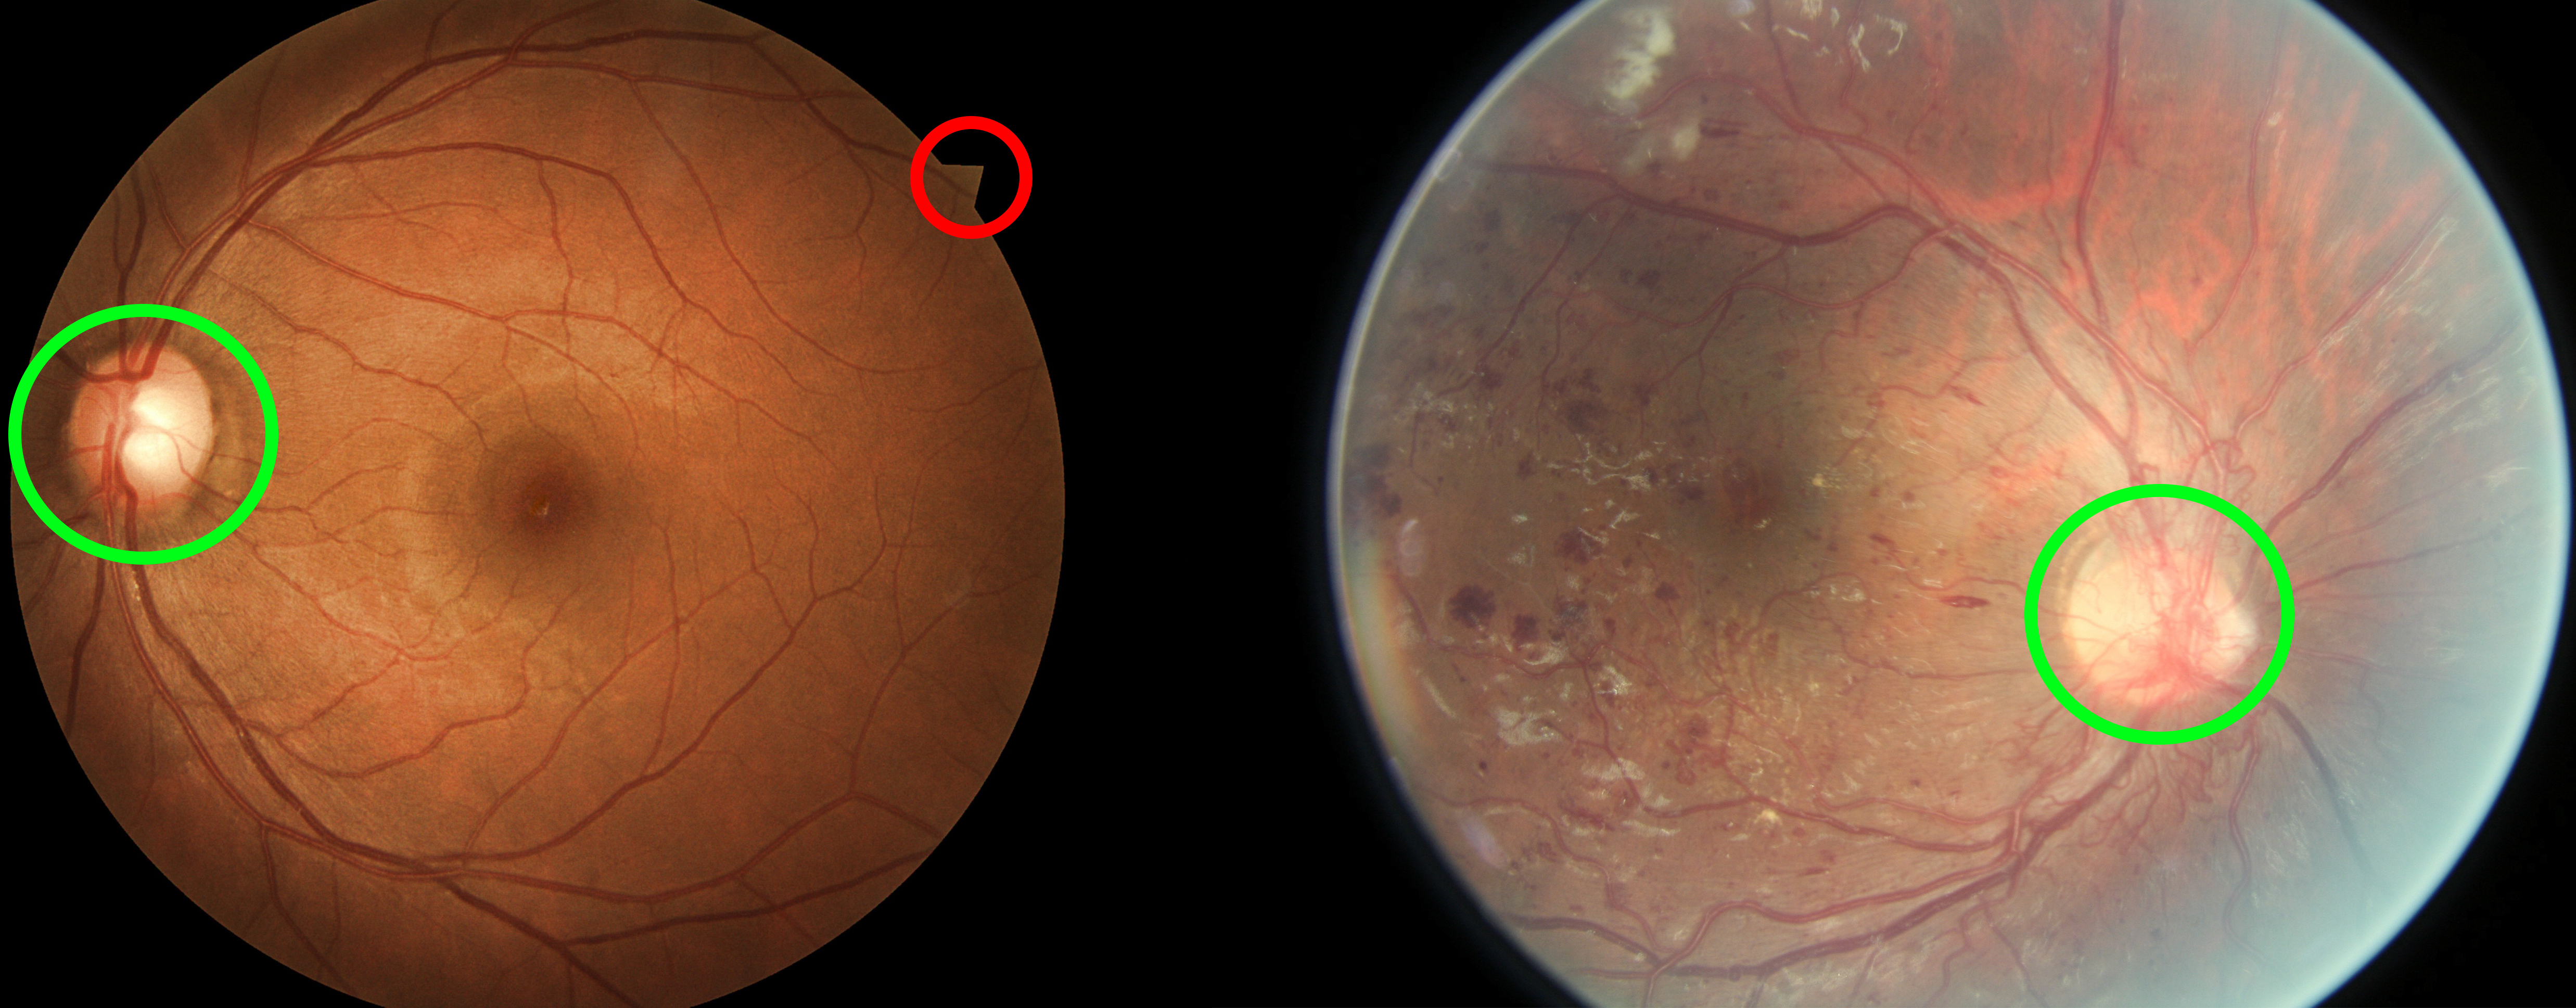
\includegraphics[width=\textwidth]{figures/chapter4/Dataset/comparison.jpg}
    \caption{Inverted and non-inverted image. Optic disk (green) and torch (red) are highlighted.}
    \label{fig:inverted}
\end{figure}

The dataset has a total of 88.704 fundus images, divided into two sets: a training set consisting of 35.126 images and a test with 53.578 files, summing a total of 88 GB. The images include the left and right eye for each of the 44.352 observed patients. 

The images come from a variety of cameras and may have different colors, resolutions, and capture different part of the eyes. Some images also contain significant noise, in the shape of under or overexposure, reflections or other graphical artifacts.

Different images may also have different orientations, depending on the type of equipment used to take the photograph. Some images are anatomically oriented (for the right eye, the macula is on the left and the optic nerve is on the right or there is a notch on the side of the image) and others are mirrored, as depicted in \Cref{fig:inverted}.

The resolution of images is quite varied: for the training set, the width of the images is between 400 and 5184 pixels with a mean of 3637 pixels and the height between 289 and 3.456 with a mean of 2.473 pixels. The relationship between width and height (the aspect ratio) is also remarkably different between images, which means the images cannot be directly resized to a common size without heavily distorting some of them.

All the images are compressed as JPEG and the image size is between 0.01 and 2.07 Megabytes with a mean of 1.03 Megabytes.

\begin{figure}[htbp]
     \begin{subfigure}[b]{0.19\textwidth}
         \centering
         \includegraphics[width=\textwidth, height=\textwidth]{figures/chapter4/Dataset/noDR/41_left.jpeg}
    \end{subfigure}
    \hfill
    \begin{subfigure}[b]{0.19\textwidth}
         \centering
         \includegraphics[width=\textwidth, height=\textwidth]{figures/chapter4/Dataset/mild/114_left.jpeg}
    \end{subfigure}
    \hfill
    \begin{subfigure}[b]{0.19\textwidth}
         \centering
         \includegraphics[width=\textwidth, height=\textwidth]{figures/chapter4/Dataset/moderate/129_left.jpeg}
    \end{subfigure}
    \hfill
    \begin{subfigure}[b]{0.19\textwidth}
         \centering
         \includegraphics[width=\textwidth, height=\textwidth]{figures/chapter4/Dataset/severe/163_left.jpeg}
     \end{subfigure}
     \hfill
     \begin{subfigure}[b]{0.19\textwidth}
         \centering
         \includegraphics[width=\textwidth, height=\textwidth]{figures/chapter4/Dataset/proliferative/294_left.jpeg}
     \end{subfigure}

    \bigskip
     \begin{subfigure}[b]{0.19\textwidth}
         \centering
         \includegraphics[width=\textwidth, height=\textwidth]{figures/chapter4/Dataset/noDR/75_right.jpeg}
         \caption{Grade 0}
    \end{subfigure}
    \hfill
    \begin{subfigure}[b]{0.19\textwidth}
        \centering
        \includegraphics[width=\textwidth, height=\textwidth]{figures/chapter4/Dataset/mild/36_right.jpeg}
        \caption{Grade 1}
    \end{subfigure}
    \hfill
    \begin{subfigure}[b]{0.19\textwidth}
        \centering
        \includegraphics[width=\textwidth, height=\textwidth]{figures/chapter4/Dataset/moderate/54_right.jpeg}
        \caption{Grade 2}
    \end{subfigure}
    \hfill
    \begin{subfigure}[b]{0.19\textwidth}
        \centering
        \includegraphics[width=\textwidth, height=\textwidth]{figures/chapter4/Dataset/severe/326_right.jpeg}
        \caption{Grade 3}
     \end{subfigure}
     \hfill
     \begin{subfigure}[b]{0.19\textwidth}
        \centering
        \includegraphics[width=\textwidth, height=\textwidth]{figures/chapter4/Dataset/proliferative/352_right.jpeg}
        \caption{Grade 4}
    \end{subfigure}
    \caption{Example of images of different classes. Note the different color, brightness, and scale of each image. }
    \label{fig:disease_level}
\end{figure}

Both train and test images have been graded for DR by a professional ophthalmologist: the rating is a number between 0 and 4 representing no DR, mild, moderate or severe DR or proliferative DR. The  \Cref{fig:disease_level} shows some examples of images in each of these classes.

\begin{table}[tb]
\centering
\begin{tabular}{|c|c|c|}
\hline
Disease Stage                                                        & Number of Images & Proportion \\ \hline
\hline
\begin{tabular}[c]{@{}c@{}}No apparent \\ retinopathy\end{tabular}   & 25.810            & 73.48\%    \\ \hline
Mild retinopathy                                                     & 5.292             & 15.06\%    \\ \hline
\begin{tabular}[c]{@{}c@{}}Moderate \\ retinopathy\end{tabular}      & 2.443             & 6.95\%     \\ \hline
\begin{tabular}[c]{@{}c@{}}Severe \\ retinopathy\end{tabular}        & 873              & 2.49\%     \\ \hline
\begin{tabular}[c]{@{}c@{}}Proliferative \\ retinopathy\end{tabular} & 708              & 2.02\%     \\ \hline
\end{tabular}
\label{table:classDistribution}
\caption{Distribution of classes in the
dataset. No DR cases are heavily overrepresented}
\end{table}
Concerning class distribution, the dataset is heavily unbalanced, as no DR images account for 73.48\% of the training set, while the Mild, Moderate, Severe and Proliferative DR have a representation of 15.06\%,  6.95\%, 2.49\% and 2.02\% respectively, as depicted in \Cref{table:classDistribution}.

There is a strong correlation between the left and right eye grading (Pearson correlation coefficient \( \rho = 0.85 \)). We find two possible causes behind this phenomenon: in the first place, persistently high sugar levels in blood should damage both retinas at a similar rate, leading to similar levels of DR. In the second place, physicians usually examine both eyes at once, so it is possible that the prediction made for one eye biases the grading of the second. Whatever the cause, it may be worth exploring \textit{binocular} methods, that consider information coming from both eyes for grading.

\section{Preprocessing}
While most CNN models can work with a wide set of image sizes, using a very high resolution is not computationally feasible, especially in the face of limited computational power. Instead of just resizing them, it is convenient to first crop the background, as it provides no information.

However, detecting the background is not straightforward, as its color may differ between images (although it's dark in all cases). Most naive strategies we tried (as detecting the color of the corners) failed in a subset of cases, for example, when the eye is significantly zoomed.

We finally chose a scheme heavily inspired by the one carried by the winner of the Kaggle competition Ben Graham \cite{competitionRep}, consisting in 3 steps implemented using the open source libraries OpenCV \cite{openCv} and Pillow \cite{pillow}:
\begin{enumerate}
    \item \textbf{Scale down the image, so the radius has a fixed length}: to do this, we first identify the background by drawing a horizontal line through the center of the image and reducing each pixel to the sum of the three RGB components.

    Since the background is close to black, the sum of its pixels will have a very low value. We discard them by selecting the pixels whose components sum more than one tenth of the mean sum.

    The resulting line mostly corresponds to the diameter of the eye. We resize both the x and y-axis by a constant factor, so the radius has 300 pixels. The size of the radius should be adjusted depending on the working resolution of choice.
    
    \item \textbf{Overlap Gaussian noise over the image}: Gaussian noise is created by applying a convolution to the image with a Gaussian kernel, a kernel created by extracting values from a \( \normal(\eta = 0, \sigma = 10) \) distribution, which can be readily done using \( \texttt{gaussianBlur} \) method from OpenCV. 

    We then combine the original and the blurred images using an affine combination, so the final image is equal to \( \alpha I_0 + \beta I_G + \gamma \), where \( I_0 \) is the original image, \( I_G \) the blurred one and \( \alpha = 4, \beta = -4, \gamma = 128\) (the operation is applied independently for each channel). This operation can be done using the \( \texttt{addWeighted} \) method from OpenCV.

    Since \( I_G \) is the blurred version of the original image, the operation is approximately similar to subtracting the local average color. Pixels with a color similar to average one will become gray (color (128, 128, 128)) while pixels with a color different from the surrounding one will remain distinctive. This is especially useful to highlight blood vessels and lesions. 
    
    \item \textbf{Homogenize the background and crop}: we draw a circle in the center of the image, with radius equal to \( 0.9 \) times the radius of the eye (300 pixels). We then set all the pixels outside the circle to a constant color (128, 128, 128).

    To crop the background it is now sufficient to select the smallest bounding box containing all pixels different from the background color, which is straightforward using the \texttt{bbox} method from Pillow.
\end{enumerate}


\begin{figure}[tb]
     \begin{subfigure}[b]{0.24\textwidth}
         \centering
         \includegraphics[width=\textwidth, height=\textwidth]{figures/chapter4/Preprocessing/original.jpg}
         \caption{Original}
    \end{subfigure}
     \hfill
         \begin{subfigure}[b]{0.24\textwidth}
        \centering
        \includegraphics[width=\textwidth, height=\textwidth]{figures/chapter4/Preprocessing/blurred.jpg}
        \caption{Blurred}
    \end{subfigure}
    \hfill
     \begin{subfigure}[b]{0.24\textwidth}
        \centering
        \includegraphics[width=\textwidth, height=\textwidth]{figures/chapter4/Preprocessing/weighted.jpg}
        \caption{Overlapped}
    \end{subfigure}
    \hfill
     \begin{subfigure}[b]{0.24\textwidth}
        \centering
        \includegraphics[width=\textwidth, height=\textwidth]{figures/chapter4/Preprocessing/cropped.jpg}
        \caption{Cropped}
    \end{subfigure}
    \caption{Process of preprocessing an image. The original image is rectangular, so it appears stretched when scaled to a squared image.}
    \label{fig:completePreprocess}
\end{figure}

The technique of adding Gaussian noise to images is a common technique in data augmentation, as it can make small details stand up and well-behaved noise can help the model become more robust. 

In its current shape, it behaves as a stochastic way to achieve local histogram normalization and in our proofs it has shown superior to other techniques, such as CLAHE \cite{pizer1987adaptive}. 

\Cref{fig:completePreprocess} shows the entire preprocessing process for an image, except for changes in scale. The application of Gaussian noise successfully highlights the blood vessels and the main anatomical structures, as the optic nerve. It also removes some undesirable effects, as the changes in brightness.

After the cropping process, the image can be scaled to a square without significant stretching, which is crucial since the model should be fed similarly sized images and as we said, the original images have remarkable different aspect ratios.

\Cref{fig:preprocess} shows the result of preprocessing several images. We note that the preprocessing brings out the lesions and the pathological stretch marked pattern and provide uniform results when applied to images with very different scales and light conditions.

While this method sacrifices most color information, we have found that color is dependent on the brightness conditions and does not contain diagnostic information by itself.

\begin{figure}[tb]
     \begin{subfigure}[b]{0.24\textwidth}
         \centering
         \includegraphics[width=\textwidth, height=\textwidth]{figures/chapter4/Preprocessing/Ori/36_left.jpeg}
    \end{subfigure}
    \hfill
    \begin{subfigure}[b]{0.24\textwidth}
         \centering
         \includegraphics[width=\textwidth, height=\textwidth]{figures/chapter4/Preprocessing/Prep/36_left_prepr.jpeg}
    \end{subfigure}
    \hfill
    \begin{subfigure}[b]{0.24\textwidth}
         \centering
         \includegraphics[width=\textwidth, height=\textwidth]{figures/chapter4/Preprocessing/Ori/114_right.jpeg}
    \end{subfigure}
    \hfill
    \begin{subfigure}[b]{0.24\textwidth}
         \centering
         \includegraphics[width=\textwidth, height=\textwidth]{figures/chapter4/Preprocessing/Prep/114_right.jpeg}
     \end{subfigure}

    \bigskip
     \begin{subfigure}[b]{0.24\textwidth}
         \centering
         \includegraphics[width=\textwidth, height=\textwidth]{figures/chapter4/Preprocessing/Ori/41_left.jpeg}
    \end{subfigure}
    \hfill
    \begin{subfigure}[b]{0.24\textwidth}
        \centering
        \includegraphics[width=\textwidth, height=\textwidth]{figures/chapter4/Preprocessing/Prep/41_left_crop.jpeg}
    \end{subfigure}
    \hfill
    \begin{subfigure}[b]{0.24\textwidth}
        \centering
        \includegraphics[width=\textwidth, height=\textwidth]{figures/chapter4/Preprocessing/Ori/294_left.jpeg}
    \end{subfigure}
    \hfill
    \begin{subfigure}[b]{0.24\textwidth}
        \centering
        \includegraphics[width=\textwidth, height=\textwidth]{figures/chapter4/Preprocessing/Prep/294_left.jpeg}
     \end{subfigure}

    \bigskip
     \begin{subfigure}[b]{0.24\textwidth}
         \centering
         \includegraphics[width=\textwidth, height=\textwidth]{figures/chapter4/Preprocessing/Ori/54_right.jpeg}
         \caption{Original}
    \end{subfigure}
    \hfill
    \begin{subfigure}[b]{0.24\textwidth}
        \centering
        \includegraphics[width=\textwidth, height=\textwidth]{figures/chapter4/Preprocessing/Prep/54_right.jpeg}
        \caption{Processed}
    \end{subfigure}
    \hfill
    \begin{subfigure}[b]{0.24\textwidth}
        \centering
        \includegraphics[width=\textwidth, height=\textwidth]{figures/chapter4/Preprocessing/Ori/352_right.jpeg}
        \caption{Original}
    \end{subfigure}
    \hfill
    \begin{subfigure}[b]{0.24\textwidth}
        \centering
        \includegraphics[width=\textwidth, height=\textwidth]{figures/chapter4/Preprocessing/Prep/352_right.jpeg}
        \caption{Processed}
     \end{subfigure}
    \caption{Result of preprocessing. It can be observed details like capillaries or lesions have
become more obvious and most of the illumination artifacts have disappeared.}
    \label{fig:preprocess}
\end{figure}

\section{Data augmentation}
Since we have limited data, it is convenient to use data augmentation techniques to create small variations of images. This will not only increase the effective size of the dataset, but also prevent overfitting and increase the robustness of the model.

By randomly applying transformations to an image before feeding them into the model, the model can become robust against rotations, reflections, or color variations of the images. We apply the following transformations (from the Albumentations open source library \cite{albumentations}) to each image with probability \( 0.5 \): scaling the image by a random factor in  \( (0.9, 1.1) \), rotating it by a random angle, flipping it vertically, horizontally or both. We do not include color or brightness transformation, as the preprocessing method removes the main of both from the original image. After this process, the image is scaled to the working resolution, that will usually depend on the concrete choice of the model.

To be able to process the images it is convenient that they are (approximately) normalized, so all components have a similar magnitude and the learning process is not affected by spurious differences of scales.

We apply normalization after data augmentation and immediately before feeding the image to the model. The normalized image \( I' \) is calculated from the augmented image \( I \) as:
\[I' = \frac{I - \mu}{\sigma}\]
where \( \mu \) is the mean and \( \sigma \) is the standard deviation, calculated separately for each channel over the whole training set. 
    \chapter{CNN classifier using transfer learning}\label{chapter5}
In order to choose a CNN model, we evaluated several contemporary architectures, as ResNeXt \cite{xie2017aggregated} or ConvNeXt \cite{liu2022convnet} and finally opted for an EfficientnetV2 architecture \cite{tan2021efficientnetv2}, a general purpose architecture proposed by Google researchers that showed excellent performance.

We present the design ideas behind the EfficientNet architecture and its adaptation to our current problem. We also evaluate the results of the model and some additional properties, like calibration.

\section{The EfficientNet architecture} \label{sec:efficientnet}
EfficientNet \cite{efficientNet, googleEfficient} is a family of models that emerged to improve the efficiency and accuracy of existing models by scaling an established model. It is common to scale convolutional neural networks once more resources are available, in order to improve performance. The conventional way to scale these models is to arbitrarily increase the different dimensions of the network, either the depth or the width or the resolution.

Unlike conventional methods, EfficientNet uses a novel way of scaling the model by uniformly resizing each dimension based on a fixed set of scaling coefficients. This strategy is very successful as EfficientNet significantly outperformed the state-of-art models.

The key of this model is to scale all the dimensions of the neural network (\Cref{fig:scaling}). In order to achieve this, an exhaustive search of the hyperparameters of the network is carried out to find the relationship between different scaling orders of each dimension in the base model under a set of restrictions. Once this search is performed, the scaling coefficient for each dimension is determined.

 \begin{figure}[tb]
    \centering
    \includegraphics[width=\textwidth]{figures/chapter5/efficient/compoundScaling.png}
    \caption{Difference between traditional techniques for scaling CNNs (b), (c), (d) and the scaling method used by EfficientNet (e) \cite{efficientNet}.}
    \label{fig:scaling}
\end{figure}
The choice of the base model (a) is crucial. EfficientNet uses a technique for automating the design of artificial neural networks called Neural Architecture Search (NAS) \cite{white2023neural}, consistent in searching the model that maximizes a performance estimation over a predefined family of models. The result of this search is EfficientNet-B0, whose architecture is presented in \Cref{fig:baseline}. The rest of the models of the family are created by scaling the baseline using the previously found hyperparameters: the original family consisted of 7 additional models (from B1 to B7) ranging from the 5.3 million parameters of the backbone to 66 millions parameters for B7.

\begin{figure}[tb]
    \centering
    \includegraphics[width=\textwidth]{figures/chapter5/efficient/EfficientNetv0.png}
    \caption{Baseline Architecture}
    \label{fig:baseline}
\end{figure}

Presented in 2021, EfficientNetV2 proposes an improvement over the EfficientNet family, achieving higher parameter efficiency and higher training speed than other previous models and comparing favorably against much bigger vision transformer models such as ViT-L (\Cref{fig:comparison}). 
\begin{figure}[tbp]
    \centering
    \includegraphics[width=0.6\textwidth]{figures/chapter5/efficient/graficaV2.png}
    \caption{Comparison with other models: EfficientNetV2 obtains better accuracy with a fraction of parameters and training time \cite{tan2021efficientnetv2}.}
    \label{fig:comparison}
\end{figure}

The creators of EfficientNetV2 maintained the original objective of EfficientNet: maximizing the parameter efficiency, in order to obtain state-of-the-art results with relatively small models. The v2 version pays especial attention to the problem of training, as the EfficientNet models required careful hyperparameter tuning and were not especially fast to train. EfficientNetV2 is up to 11 times faster training speed and 6.8 times more parameter efficiency in ImageNet, CIFAR, Cars and flowers datasets than the state of the art models \cite{tan2021efficientnetv2}, a speed-up that becomes more notable when using large resolution images.

The models of the v2 family are therefore excellent candidates for situations with limited computing power. The team designed the architecture around the main bottlenecks of EfficientNet. They found the following problems \cite{tan2021efficientnetv2}:

\begin{enumerate}
    \item Training using very large images is slow: EfficientNet's utilization of large image size results in significant memory usage. To alleviate the problem they propose to use \textit{progressive learning}, which involves progressively increasing the image size provided to the model. This approach exploits the fact that the use of global pooling makes the model agnostic about the input size.
    \item Depthwise convolutions show slower performance in the initial layers, but they are effective in later stages: these type of convolutions have fewer parameters and require fewer floating point operations per second compared to regular convolutions, but they often fail to fully leverage the capabilities of modern accelerators. The researchers proposed to alternate the use of different convolutional blocks (as Fused-MBconv and MBConv) and perform Neural Architecture Search to find the best combination to maintain the efficiency in parameters and make training faster.
    \item Scaling up each stage equally is suboptimal: EfficientNet scales all stages uniformly using a simple rule, but the stages don't contribute equally to the training speed or parameter efficiency.  However, EfficientNetsV2 use a non-uniform scaling strategy to progressively add more layers to the later stages. 
\end{enumerate}

The result of these improvements was a complete family of models comprising both minimal models (like EfficientNetV2-B0 with just 7.4 million of parameters) and very large models (like EfficientNetV2-XL, which has 208 million parameters).

\section{Model Architecture}\label{archModel}
The usual architecture for a vision model for classification is composed of a \textit{backbone} and a \textit{classifier}. The \textit{backbone} works as a \textit{feature extractor} that will encode the input into a feature representation. In the case of a convolutional neural network, the backbone is usually composed of a convolutional block and a \textit{global pool layer}, that will determine how the hidden channels of the representation are merged.

The \textit{classifier} is often a conventional neural network and can be substituted for other components to address other problems, usually maintaining the original backbone.

We will follow a similar architecture: the backbone of our model (\Cref{fig:architecture}) is an EfficientNetV2-B3 model, a medium-sized (14M parameters) architecture that presents a good compromise between accuracy and complexity. We used the implementation from the open source library timm \cite{timm} (Pytorch Image Models). 

Furthermore, we opted for a working resolution of 512 × 512, offering a good compromise between performance and efficiency. 

\begin{figure}[ht]
    \centering
    \includegraphics[scale=0.3]{figures/chapter5/models/model.png}
    \caption{Architecture of the model. The features extracted by the CNN are pooled using global average pooling before being flattened and fed to the classifier.}
    \label{fig:architecture}
\end{figure}

The backbone is fed each image and its output is pooled using \textit{global average pooling}, which reduces each channel of the output to a single scalar, by averaging all the components of the channel. We use as classifier a simple linear network which outputs the \textit{logits}, the unnormalized probabilities for each class.

\subsection{Transfer learning}
Since we were restricted to models that could be trained with limited computational resources, we opted to use a CNN and to apply transfer learning: using a model trained for one task (in the case of CNN, usually object detection in a general purpose dataset as ImageNet) and retrain it for a new task over the specific dataset (\textit{fine-tuning}).

Transfer learning has been proved to be a reliable way to save computational power even in the case that the original and the new datasets are quite different, apparently because features originally learned can be reused \cite{haslum2022makes}.

We use a backbone pretrained on ImageNet21K, a database with 21,000 general purpose images for image classification problems. In order to not destroy the original weights, we \textit{fine-tune} the model to the new database using a low learning rate. We opted for training the whole model (without freezing any layer), since the ImageNet database is quite different to the EyePACS one.

In our experiments, the pretrained model obtained an accuracy of 83.5\% after just one iteration, compared to just 52.6\% for the non-pretrained one, which suggests transfer learning is highly successful at reducing training time and easing convergence with almost none overhead.

\subsection{Training the model}
The model was trained using Adamax optimizer \cite{kingma2017adam} and unweighted Cross Entropy as the loss function. \Cref{table:adamax} shows the hyperparameters of the optimizer used for training, so the results can be reproduced.

We tried other strategies as alternative optimizers (Adam, SGD) as well as approaching the problem as a regression, but they offered poorer results. We did not find reliable strategies to improve the performance over under-represented classes. Both oversampling (showing the model more images from under-represented classes each epoch) and under-sampling (reducing the number of over-represented classes in the dataset) severely deteriorated performance both general and over under-represented classes. 

Weighting under-represented classes (so the loss for instances of underrepresented classes is weighted more than for instances of over-represented classes) also weakened the model performance.

\begin{figure}[tb]
     \begin{subfigure}[b]{0.65\textwidth}
        \centering
        \includegraphics[width=\textwidth]{figures/chapter5/metrics/loss.png}
        \caption{Loss evolution during training.}
        \label{fig:training}
    \end{subfigure}
    \hfill
    \begin{subfigure}[b]{0.34\textwidth}
        \centering

        \resizebox{\columnwidth}{!}{
        \small
        \begin{tabular}{|cc|}
        \hline
        \multicolumn{2}{|c|}{Hyperparameters: Adamax} \\ \hline \hline
        Lr & 1e-2 \\ \hline
        $(\beta_1, \beta_2)$  & (0.9, 0.999)  \\  \hline
        $\epsilon$ & 1e-7 \\  \hline
        Weight decay & 1e-2 \\ \hline
        \end{tabular}
        }
        \caption{Hyperparameters used for training.}
        \label{table:adamax}
    \end{subfigure}
\end{figure}

We trained for 50 epochs in an Nvidia GTX 1070 GPU (approximately 9 hours). The results of training are shown in \Cref{fig:training}. We observed very fast convergence during the first epoch followed by \textit{overfitting}, that we addressed adding regularization in the form of weight decay and late dropout \cite{liu2023dropout} and reducing the learning rate, achieving model convergence. The evolution of the main indicators (accuracy, macro F1 and Cohen's Kappa coefficient) led us to think the model has a good performance in all classes. 

As it is common in the field, we used Cohen's kappa coefficient as the main measure of performance. This statistic estimates the accuracy of a rating by comparing it with the expected accuracy of a random rater \cite{cohen1960kappa}. 

\begin{figure}[tb]
     \centering
     \begin{subfigure}[b]{0.32\textwidth}
         \centering
         \includegraphics[width=\textwidth]{figures/chapter5/metrics/accuracy.png}
         \caption{Accuracy}
         \label{fig:accuracy}
     \end{subfigure}
     \hfill
     \begin{subfigure}[b]{0.32\textwidth}
         \centering
         \includegraphics[width=\textwidth]{figures/chapter5/metrics/f1.png}
         \caption{F1 score}
         \label{fig:f1}
     \end{subfigure}
     \hfill
     \begin{subfigure}[b]{0.32\textwidth}
         \centering
         \includegraphics[width=\textwidth]{figures/chapter5/metrics/kappa.png}
         \caption{Cohen's $\kappa$}
         \label{fig:kappa}
     \end{subfigure}
        \caption{Performance of the model during training, measured by three metrics: accuracy, macro F1 score and squared Cohen kappa}
        \label{fig:metrics}
\end{figure}

\subsection{Calibrating the model}
In order to carry further analysis, it is convenient to be able to interpret the predictions of the model in terms of probabilities for each class.

It has been observed that most deep learning models tend to be overconfident and directly interpreting the results of the model as probabilities (by applying \textit{softmax} to the logits) will not reflect the true likelihood of the event \cite{guo2017calibration}.

In a well calibrated model, the probability associated with the predicted class label reflects its ground truth correctness likelihood.

To calibrate the model we use \textit{temperature scaling} \cite{guo2017calibration}, a method which estimates a constant \( T \) to scale the logits output by the model to minimize negative log likelihood over the validation set. After regularization, the probability of the classes is given by \( p = \softmax(y / T) \) where \( y \) are the logits of the model. In particular, temperature scaling does not affect the predictions made by the model as it does not alter the ratio between logits for different classes.

We used the implementation provided by the team responsible for the popularization of temperature scaling \cite{guo2017calibration}, which employs a neural network to estimate a value of \( T = 1.15 \).

\begin{figure}[tbp]
    \centering
    \includegraphics[scale = 0.45]{figures/chapter5/calibration/post_calibration.png}
    \caption{Reliability diagram after calibration. }
    \label{fig:reliability}
\end{figure}

The reliability diagram after normalization (\Cref{fig:reliability}) shows that the final model is relatively well calibrated and is quite precise for high levels of accuracy, although the model tends to be too unconfident about cases with low accuracy. 

The estimated calibration error (the expected value of the gap between confidence and accuracy) is just 0.02, which confirms the model is indeed well-calibrated.

We can use the calibrated probabilities to identify images that are particularly challenging to grade for the model (\Cref{fig:unconfident}). While some of these images are too noisy to be useful (\Cref{fig:unconfident0}), others pose a real challenge because of unusual framing or coloring, like \Cref{fig:unconfident3}. 

There are multiple use cases for images like these: for example, to test the performance of preprocessing methods over images with unusual characteristics or to implement educational tools for ophthalmology students. 

\begin{figure}[tb]
     \centering
     \begin{subfigure}[b]{0.32\textwidth}
         \centering
         \includegraphics[height=\textwidth,width=\textwidth]{figures/chapter5/unconfident/10345_right.jpeg}
         \caption{Pred.: 1. Target: 2}
         \label{fig:unconfident0}
     \end{subfigure}
     \hfill
     \begin{subfigure}[b]{0.32\textwidth}
         \centering
         \includegraphics[height=\textwidth,width=\textwidth]{figures/chapter5/unconfident/3042_left.jpeg}
         \caption{Pred.: 0. Target: 2.}
     \end{subfigure}
     \hfill
    \begin{subfigure}[b]{0.32\textwidth}
         \centering
         \includegraphics[height=\textwidth,width=\textwidth]{figures/chapter5/unconfident/35800_right.jpeg}
         \caption{Pred.: 2. Target: 2}
        \label{fig:unconfident3}
     \end{subfigure}
    \caption{Some images predicted with lower confidence (\( \leq 35\%\)) }
    \label{fig:unconfident}
\end{figure}

\subsection{Blending information from both eyes} \label{sec:blending} 
As we observed when exploring the dataset, there is high correlation between the DR grading of the left and right eye. We can use that correlation to \textit{blend} information coming from both eyes to create a prediction for each eye.

After trying different strategies for blending (as combining predictions from both eyes using a dedicated neural network) we opted for a feature-level approach, depicted in \Cref{fig:blended_model}.

In this approach, we use the CNN as a feature extractor for the left and right eye images. These features are concatenated and fed to a dense neural network, which generates a prediction for each eye. Compared to prediction-level blending, this strategy allows the classification of one eye to directly depend on features extracted on another eye.

We found that the strategy of using CNN as a feature extractor and adding detachable heads offered powerful and flexible solutions to different problems as blending or embedding extraction. Since heads are usually simple networks, they can be trained fast without significant computing cost.

In order to prevent overfitting, we used a heavily regularized network including \textit{dropout} after every layer and using LeakyReLU as an activation function. Blending both eyes' information provides a slight improvement over the simple classifier, increasing Kappa score by 0.018 points (from 0.80 to 0.818).

\begin{figure}[tb]
    \centering
    \includegraphics[scale=0.35]{figures/chapter5/models/blended_model.png}
    \caption{Architecture of the model for feature blending}
    \label{fig:blended_model}
\end{figure}

We also found that a slight improvement could be achieved by using a more sophisticated way to generate a class prediction from the model output. The result of processing an image is the (post-calibration) vector of logits \( y \), which represents the unnormalized probability for each class. Until this point, we generated the prediction as the class associated to the higher probability, which is especially convenient for validation, since this is a very fast process.

These probabilities can be normalized by applying \textit{softmax}. We then calculate the value \( \sum_{i = 0}^4 i y_i \) and obtain the prediction using a set of precomputed thresholds (0.57, 1.37, 2.30, 3.12), that we identified as providing the best \( \kappa \) score on the validation set using exhaustive search. Using this technique to generate predictions increased the \( \kappa \) score to 0.844, a very significant improvement.

To generate the final predictions we fed the model the test images by left and right pairs, each one rotated by a random angle and created five independent predictions. We obtained the final prediction by calculating \( \sum_{i = 0}^4 i \softmax(y_i^k) \) for each of the \( y^1, \dots, y^k \) vector of logits, averaging the results and using the previously found thresholds. We obtained a final kappa value of \( \kappa = 0.8491 \), which shows that generating multiple predictions is effective at improving performance.

\section{Model evaluation}
The obtained \( \kappa \) value would set us 2nd (out of 660 competitors) in the Kaggle competition for Diabetic Retinopathy Detection \cite{diabeticretinopathydetection}, which used the same setting. The first solution has a \( \kappa \) coefficient superior by less than \( 0.0005 \) and used an ensemble of three models, as almost all the dominant solutions did. While ensembles are a reliable way to improve performance, they are inconvenient since they increase training costs and, what is more important, multiply the time and resources needed for inference.

Our approach shows the viability of using pretrained smaller models to obtain excellent results in a computationally efficient way. The ROC curve, displayed in \Cref{fig:roc}, shows promising results with an area under the curve of 0.87 for referable cases (some sign of diabetic retinopathy) and 0.88 for severe cases (at least grade 3). 

\begin{figure}[tb]
     \centering
     \begin{subfigure}[b]{0.49\textwidth}
        \centering
        \includegraphics[width=\textwidth,height=.9\textwidth]{figures/chapter5/roc.png}
        \caption{ROC curve for referable cases (at least grade 1) and severe cases (at least grade 3)}
        \label{fig:roc}
     \end{subfigure}
     \hfill
     \begin{subfigure}[b]{0.49\textwidth}
        \includegraphics[width=\textwidth,height=.9\textwidth]{figures/chapter5/confusion.png}
        \caption{Confusion matrix for the obtained predictions}
        \label{fig:confusion}
     \end{subfigure}
     \hfill

    \centering
\end{figure}

The final level of accuracy is \( 83.31 \% \). The confusion matrix obtained is shown in \Cref{fig:confusion}. The performance is excellent over class 0 and reasonable solid over classes 2, 3 and 4. The difficulty to correctly detect the disease at grade \( 1 \) is in line with previous observations in the field about the complexity of correctly diagnosing intermediate classes. 

We must stress that the election of the thresholds for generating the final classification was intended to maximize the \( \kappa \) value, and they can and should be adjusted before applying the model to clinical practice, for example to reduce the rate of false negatives for grade 1 images.
    \chapter{Similar case retrieval for DR diagnosis} \label{chapter6}
In this section we explore another way of using the model in a clinical context beyond mere DR grading: showing the clinician images with similar diagnostic features to help them diagnose a new case. The contents of this section were developed in cooperation with the director of this work, Professor Antonio Alejandro Sánchez Ruiz-Granados, as a part of an article for the International Conference on Case-Based Reasoning. 

\section{Extraction of \textit{embeddings}}
An important part of the expressiveness of neural networks comes from their ability to create low-dimensional representations of the data containing most of the information necessary for the task at hand; these representations are called \textit{embeddings}. Indeed, the output of the global average pooling of the convolutional component of the network (which is a real vector with 1.536 components) must contain most the information necessary to evaluate the DR grading of the image, since this is all the information the classifier is fed. 

In a model like the one depicted in \Cref{fig:architecture}, the classifier is a purely linear component, so different classes must lie in linearly separable components of the space: this means we can use the spatial structure of the embeddings to obtain semantic information about the fundus images.

\begin{figure}[tb]
    \centering
    \includegraphics[scale=0.2]{figures/chapter6/model_head.png}
    \caption{Structure of the model after adding a new multilevel classifier. The first two layers are regularized using dropout (\( p = 0.3\)). All the layers use Leaky ReLU (\( \alpha = 0.5 \)) except for the last one, that is purely linear. }
    \label{fig:model_headed}
\end{figure}

However, we found that these embeddings were too high dimensional to be used efficiently and applying generic dimensionality reduction techniques (UMAP, t-SNE or PCA) returned low-quality results. To overcome this problem we extended the classifier adding three regularized fully connected layers (\Cref{fig:model_headed}), serving as a context-aware dimensionality reduction of data. We chose to progressively reduce the width of layers by a factor of \( 4 \), so we had access to embeddings of different dimensionality. In order to save computational power, we reused the convolutional block and retrained the new layers.

In order to visualize embeddings we extracted the input of the \texttt{fc4} layer to obtain 32-dimensional features. Since this is the final linear layer,  these embeddings preserve the aforementioned property of linear separability by class. Extracting the input of previous layers gives us access to additional embeddings for each image, of dimensions 1536, 384 and 96. 

\Cref{fig:embedding}, shows a visualization of the 32-dimensional embeddings for a sample of 3,000 points, projected to the plane using UMAP \cite{mcinnes2018umap} and labelled both by predicted and target class. The image leads us to two relevant assertions: \begin{enumerate*}[label=(\arabic*)]
\item the network successfully creates a representation of the input image that spatially encodes diagnostic information of the disease and \item the spatial structure is robust enough to persist after severe dimensionality reduction\end{enumerate*}. 

\begin{figure}[tb]
     \centering
     \begin{subfigure}[b]{0.49\textwidth}
         \centering
         \includegraphics[width=\textwidth]{figures/chapter6/embeddings/embeddings_predicted.png}
         \caption{Embeddings by predicted class}
         \label{fig:embedding_predicted}
     \end{subfigure}
     \hfill
     \begin{subfigure}[b]{0.49\textwidth}
         \centering
         \includegraphics[width=\textwidth]{figures/chapter6/embeddings/embeddings_target.png}
         \caption{Embeddings by target class}
         \label{fig:embedding_target}
    \end{subfigure}
    \caption{Projection into the plane of the 32-dimensional features using UMAP. }
    \label{fig:embedding}
\end{figure}

\begin{figure}[tb]
     \centering
     \begin{subfigure}[b]{0.49\textwidth}
        \centering
        \includegraphics[width=\textwidth]{figures/chapter6/embeddings/hit_miss.png}
        \caption{Projected embeddings labelled by hit/miss on the original image (DR grade was correctly predicted)}
        \label{fig:hit_miss}
     \end{subfigure}
     \hfill
     \begin{subfigure}[b]{0.49\textwidth}
        \includegraphics[width=\textwidth]{figures/chapter6/embeddings/isolated.png}
        \caption{Projected embeddings labelled by isolation (distance to the closest point is over two standard deviations of the average distance)}
        \label{fig:isolated}
     \end{subfigure}
     \hfill
    \caption{Projections of the embeddings of a sample (N = 5,000) from the train dataset, labelled by hit/miss and isolation}
    \label{fig:embeddings_explore}
    \centering
\end{figure}


\Cref{fig:hit_miss} explores the distribution of embeddings of wrongly predicted images. These images concentrate over some small regions of the space of the embeddings, which can be used to classify ``high risk'' areas, where the performance of the model may be suboptimal. Interestingly, these zones mostly coincide with the areas of distribution of isolated points (\Cref{fig:isolated}), characterized as those points which distance to the closest point is over two standard deviations the average one. 

In order to further test our assertions, we implemented a k-NN classifier using the 96-dimensional embeddings and different metrics. The class is obtained as the weighted average of the neighbors, weighted by the inverse of the distance. 

The results, shown in \Cref{table:knn}, are impressively solid, achieving even a higher accuracy than the neural network for some choices of \( k \) and a reasonable value for Cohen's \( \kappa \). The results are robust between metrics and choices of \( k \) but using other dimensions for the embeddings severely degraded performance, which reinforces the importance of using adequately sized embeddings for each task. 

\begin{table}[tb]
    \centering
    \small
    \begin{tabular}{c|cccccc|}
    \cline{2-7}
        & \multicolumn{2}{c|}{k = 3} & \multicolumn{2}{c|}{k = 11} & \multicolumn{2}{c|}{k = 15} \\ \cline{2-7} 
        & Accuracy & \multicolumn{1}{c|}{$\kappa$} & Accuracy & \multicolumn{1}{c|}{$\kappa$} & Accuracy & \multicolumn{1}{c|}{$\kappa$} \\ \hline \hline
    \multicolumn{1}{|c|}{Manhattan} & 0.8322 & \multicolumn{1}{c|}{0.7810} & 0.8437 & \multicolumn{1}{c|}{0.7945} & 0.8439 & 0.6078 \\ \hline
    \multicolumn{1}{|c|}{Euclidean} & 0.8324 & \multicolumn{1}{c|}{0.7825} & 0.8439 & \multicolumn{1}{c|}{0.7951} & 0.8440 & 0.6084 \\ \hline
    \multicolumn{1}{|c|}{Cosine} & 0.8336 & \multicolumn{1}{c|}{0.7840} & 0.8431 & \multicolumn{1}{c|}{0.7958} & 0.8425 & 0.6059 \\ \hline
    \end{tabular}
    \caption{Results obtained by a k-NN classifier ($k = 11$) on 96-dimensional embeddings}
\label{table:knn}
\end{table}

We can use the fact that the spatial structure of the embeddings contains diagnostic information to model \textit{semantic search}, the retrieval of images with similar diagnostic signs to a given one, as a \textit{nearest neighbor search} problem.

\begin{figure}[tb]
    \captionsetup[subfigure]{labelformat=empty}
     \centering
     \begin{subfigure}[b]{\textwidth}
        \begin{subfigure}[b]{0.32\textwidth}
            \centering
            \includegraphics[width=\textwidth, height=0.2\textheight]{figures/chapter6/similar/16473_right.jpeg}
            \caption{Grade 4}
         \end{subfigure}
         \hfill
         \begin{subfigure}[b]{0.32\textwidth}
            \includegraphics[width=\textwidth, height=0.2\textheight]{figures/chapter6/similar/15975_left.jpeg}
            \caption{Grade 4}
        \end{subfigure}
        \hfill
        \begin{subfigure}[b]{0.32\textwidth}
            \centering
            \includegraphics[width=\textwidth, height=0.2\textheight]{figures/chapter6/similar/3563_left.jpeg}
            \caption{Grade 4}
         \end{subfigure}
    \end{subfigure}
    \vspace{0.2em}
    
    \begin{subfigure}[b]{\textwidth}
        \begin{subfigure}[b]{0.32\textwidth}
            \centering
            \includegraphics[width=\textwidth, height=0.2\textheight]{figures/chapter6/similar/5997_left.jpg}
            \caption{Grade 0}
         \end{subfigure}
         \hfill
         \begin{subfigure}[b]{0.32\textwidth}
            \includegraphics[width=\textwidth, height=0.2\textheight]{figures/chapter6/similar/10861_right.jpeg}
            \caption{Grade 0}
        \end{subfigure}
        \hfill
        \begin{subfigure}[b]{0.32\textwidth}
            \centering
            \includegraphics[width=\textwidth, height=0.2\textheight]{figures/chapter6/similar/1669_right.jpeg}
            \caption{Grade 1}
         \end{subfigure}
    \end{subfigure}

    \caption{Two instances (one per row) of retrieval of the two most similar images to a given one (leftmost image), measuring similarity as the distance between 96-dimensional embeddings using cosine distance.}
    \label{fig:semantic_search}
    \centering
\end{figure}

\Cref{fig:semantic_search} shows the result of applying this technique to find the two images in the train set most similar to a base image from the test set, by using cosine distance to measure the distance between embeddings. We found that in 80.49\% of the cases, the image recovered as the closest one using cosine distance has the same grading as the original one and is within one level in 93\% of the cases.

As one might expect, there is an inverse correlation between the distance of the most similar image to the base and both having the same label ($\rho = -0.21$). In fact, an increase of the cosine distance between both images of \( 0.01 \), reduces the probability of both having the same grade by 50.39\% on average. 

Surprisingly, given the robustness of k-NN to the choice of metrics, we have found that different distance functions retrieved generally different images and the measured similarity of a given image can significantly vary between metrics. For example, we found that the closest image according to the cosine distance only was between the top 5 closest images according to the Euclidean distance in 38.53\% of cases. 

%----------------------------------------------------------
%
\section{Experiments and results}
\label{sec:experiments}
%
%----------------------------------------------------------

Two preliminary experiments have been conducted with the collaboration of an ophthalmologist with experience in the treatment of retinal diseases. 

The purpose of the first experiment is to check whether the similarity computed from the image embeddings is consistent with the specialist's intuition of similarity when analyzing the same images. To this end, we show the specialist 1 unlabeled base image from the test set and 5 labeled images from the training set. 

We selected the 5 images from the training set according to their similarity to the test image so that the most similar image and one in the first 4 quantiles  appear. We then asked the specialist to sort the images from the training set in order of similarity to the base image. The specialist can view all the images as many times as she wants with no time limit. This process was repeated 10 times with 10 different images from the test set. 

At the beginning of the experiment, the specialist asked what was exactly meant by ``similarity between images''. There are many criteria that can be taken into consideration: same eye (right or left), similar age of the patient, same type of lesions, same degree of DR development, images made by the same type of imaging device… 

As our neural network calculates the embeddings in the context of a system to diagnose the degree of DR, we instructed the specialist to only take into consideration lesions related to the diagnosis of that disease. Once the similarity criterion was set, the specialist made us realize that she could not sort the images corresponding to healthy eyes, as none of them had lesions. After analyzing the situation, we asked the specialist to group the images according to their similarity to the test image, but without having to order the images in the same group.

% Colorear
\begin{table}[tb]
\centering
\footnotesize
\resizebox{\columnwidth}{!}{
\begin{tabular}{|c|c|c|c|c|} 
\hline
Base & Specialist order & Embeddings order \\ 
\hline\hline
1935l  & \{1831l 4657l 12900l 27782l\} \{28227l\} & 1831l 27782l 12900l 4657l 28227l\\
20883l & \{24656l\} \{16223l 21921r 32104r 35132l\} & 24656l 35132l 21921r 32104r 16223l\\
30476r & \{11219r\} \{13843r 20464l 25222r 32358l\} & 11219r 25222r 13843r 32358l 20464l\\
31466l & \{24711r 29906r 33469l\} \{30919l\} \{10047r\} & 29906r 24711r 33469l 30919l 10047r\\
36651r & \{27153r\} \{13714r 13312l 3395r\} & 27153r 13312l 13714r 6788l 3395r\\
37151r & \{33251r\} \{329l 6569r 29141r\}  & 33251r 29141r 6569r 329l 31428l\\ 
38582r & \{7487l\} \{26381l 27973l\} \{28227l\} \{17221l\} & 7487l 27973l 26381l 17221l 28227l\\
\hline
\end{tabular}
}
\caption{Summary of the results of experiment 1. The first column contains the IDs of the base images. The second column shows the specialist's order (no order is assumed within each set). The last column shows the order according to the cosine similarity and the embeddings. Images 6788l and 31428l were discarded by the specialist due to their quality.}
\label{tab:exp1}
\end{table}

Of the 10 test images analyzed, 3 were discarded because they did not have adequate quality for diagnosis. The results of the other 7 images are shown in \Cref{tab:exp1}. In most cases, the specialist grouped the images into 2 or 3 sets using the type and number of lesions present in each image as the main criterion (her diagnosis of the degree of RD did not always match the image label). These sets should be considered as equivalence classes with no internal order but linearly ordered with respect to its similarity with the base image.

To measure the agreement between the expert's similarity ranking \[ \{ d^{(1)}_1, \dots, d^{(1)}_{n_{1}} \}, \dots, \{ d^{(m)}_1 \dots, d^{(m)}_{n_{m}} \} \]  with the order retrieved from the embeddings \( \mathcal{O} = d^{i_1}_{j_1} < d^{i_2}_{j_2} < \dots < d^{i_l}_{j_l} \), we define the cost of a transposition as \( c(d^{(i_1)}_{j_1}, d^{(i_2)}_{j_2}) = \|i_1 - i_2\| \) and calculate the sequence of transpositions of minimum cost transforming the order \( d^{(1)}_1 < d^{(1)}_2 < \dots < d^{(1)}_{n_{1}} < d^{(2)}_1 < \dots < d^{(m)}_{n_{m}}\) into \( \mathcal{O} \). 

We found this distance to be \( 0 \) in all but one case. Notably, the image retrieved as the most similar one using the embeddings is classified by the expert in the group of the most similar images in all cases, which sustains the claim that our strategy retrieves diagnostically similar images.

The purpose of the second experiment is to make a preliminary study of the usefulness and quality of the retrieved images to help the specialist in her diagnosis. To do this, we again showed the specialist the same 7 base images from the previous experiment and for each of them we followed the following protocol: (1) ask for an initial diagnosis of the image, (2) show the two most similar labeled images from the training set, (3) ask the specialist if she thought they were similar to the base image, (4) ask the specialist if it was useful to be able to see those images, and (5) ask if, in view of those images, she wanted to modify her initial diagnosis.

\begin{table}[tb]
\centering
\small
\begin{tabular}{|c|c|c|c|c|c|} 
\hline
Base & Diagnosis & Retr. tags & Similar? & Useful? & Modify diagnosis?\\
\hline\hline
1935r  & 0 & 0 0 & yes & yes & no \\	
20883l & 2 & 3 2 & yes &	yes & no \\
30476r & 3 & 3 3 & yes &	yes & no \\
31466l & 0 & 0 0 & yes & yes & no \\
36651r & 2 & 3 2 & no  & no  & no \\	
37151r & 1 & 2 1 & yes & yes & no \\	
38582r & 0 & 0 0 & yes & yes & no \\	
\hline
\end{tabular}
\caption{Summary of the results of experiment 2. The first 2 columns contain the ID of the base image to be diagnosed and its initial diagnosis. The third column show the labels of the 2 most similar images retrieved. The last 3 columns show, respectively, whether the specialist considered the retrieved images to be similar to the original one, whether being able to view those images was useful and whether, after viewing the images, she wanted to modify her initial diagnosis.}
\label{tab:exp2}
\end{table}

The results of the experiment are collected in the \Cref{tab:exp2}. The initial diagnosis of the specialist always corresponds to the label of one of the images retrieved using the embedding-based similarity and never differs by more than one degree from the other. Furthermore, in none of the cases are images of diseased eyes retrieved from healthy eyes or vice versa. All retrieved images were considered similar to the originals, except in the case of image 36651 in which the specialist indicated that the retrieved images had different type of lesions. In all other cases, the specialist considered that being able to view those similar images could be helpful for diagnostic support. In no case did the specialist modify her initial diagnosis.

Asked about the possibility of modifying the diagnosis if the system retrieved images with very different labels, the specialist said that she would continue to rely on her judgment unless the system could provide a really convincing explanation. Finally, asked about her overall impressions, she told us that she had been surprised by the system's ability to find similar images and that this feature could be useful for residents.
    \chapter{Model Interpretation} \label{chapter7}
Interpretability is crucial for medical use models. Clinical staff need to understand the way the model works in order to trust its prediction and compare it with their clinical judgment. Visualizations of the areas driving the classification can offer insights to clinicians (for example, highlighting very small lesions that could be missed) or be used as a pedagogical tool for learning clinicians. 

Interpretability techniques can also offer some guarantee against models misbehavior: for example, they may allow a clinician to identify a graphical artifact distorting classifications, as a reflection, which can make diagnosis more accurate and detect conditions of failure that can be improved. 

This chapter explores several techniques, both model specific and model agnostic, that we have implemented to explain the model previously introduced. We have tried to introduce these techniques in their context, discussing its theoretical justification and also exploring how they can help to approach lateral problems.

\section{Class activation maps}
Class activation maps are one of the preferred ways to visualize convolutional neural networks \cite{selvaraju2020grad-cam, jung2021explanations, bolei2016learning}. Suppose the last convolutional layer of the model outputs \( K \) feature maps \( A^k \in \mathbb{R}^{W \times H} \) indexed by \( i,j \).

These feature maps are then spatially pooled using Global Average Pooling and multiplied by the class weights to obtain the unnormalized probability of class \( c \):
\[
    Y^c = \sum_k w_k^c \frac{1}{Z} \sum_{i, j} A^k_{ij}
\]
where \( Z = WH \) is a normalization factor,

Since all operations involved are linear, this process is equivalent to calculating:
\[ 
    Y^c = \frac{1}{Z} \sum_{i, j} \sum_{k} w^k A^k_{ij} 
\]
but this version  includes the term \( H_{ij} = \sum_{k} w^c_k A^k_{ij} \), which expresses the result of the interaction between \( \bm{w}^c \) and \( A_{ij} \): the contribution of each part of the hidden representation to the output of \( Y^c \). We can translate this representation to an image and superimpose this term over the original input to understand which parts of the input drive the output of the model for class \( c \).

The graphic so obtained is called the \textit{class activation map} (CAM). If we fix \( c \) as the predicted class, then the CAM represents which parts of the image are the main responsible for the predicted output.

\begin{figure}[tb]
     \begin{subfigure}[b]{0.49\textwidth}
         \centering
         \includegraphics[width=0.49\textwidth,height=0.49\textwidth]{figures/chapter6/heatmaps/28699_left.png}
         \includegraphics[width=0.49\textwidth,height=0.49\textwidth]{figures/chapter6/heatmaps/28699_left_heatmap.png}
         \caption{Predicted label: 4. Target: 4.}
    \end{subfigure}
    \hfill
    \begin{subfigure}[b]{0.49\textwidth}
         \centering
         \includegraphics[width=0.49\textwidth,height=0.49\textwidth]{figures/chapter6/heatmaps/5_right.png}
         \includegraphics[width=0.49\textwidth,height=0.49\textwidth]{figures/chapter6/heatmaps/5_right_heatmap.png}
         \caption{Predicted label: 0. Target: 0.}
     \end{subfigure}

    \bigskip
    \begin{subfigure}[b]{0.49\textwidth}
         \centering
         \includegraphics[width=0.49\textwidth,height=0.49\textwidth]{figures/chapter6/heatmaps/43670_left.png}
         \includegraphics[width=0.49\textwidth,height=0.49\textwidth]{figures/chapter6/heatmaps/43670_left_heatmap.png}
        \caption{Predicted label: 4. Target: 4.}

    \end{subfigure}
    \hfill
    \begin{subfigure}[b]{0.49\textwidth}
         \centering
         \includegraphics[width=0.49\textwidth,height=0.49\textwidth]{figures/chapter6/heatmaps/43716_left.png}
        \includegraphics[width=0.49\textwidth,height=0.49\textwidth]{figures/chapter6/heatmaps/43716_left_heatmap.png}
        \caption{Predicted label: 4. Target: 4.}

     \end{subfigure}
     \centering
     \caption{Preprocessed images and class activation maps. To create the visualization we discard the bottom-50\% of the elements of the map and overlap it as pseudo-color.}
     \label{fig:heatmap}
\end{figure}

\Cref{fig:heatmap} shows both the preprocessed images and the result after overlapping the class activation map. In order to improve the readability of the result, we only preserved the top 20\% values of the CAM.

The images clearly show that the model successfully recognizes some lesions and its diagnostic importance. The map has a more disperse structures for those images with low or no DR affectation which is consistent with expectations, as these stages are characterized precisely by the absence of lesions.

There are two main problems with this approach, both related to the fact that the dimensions \( W, H \) is usually quite small (in this case, \( W = H = 16 \)). Because of repeated convolutions and pooling, each component \( H_{ij} \) summarizes information from a relatively large part of the image (a \( 32 \times 32 \) square in this case) and class activation maps won't be able to distinguish between the relative importance of objects contained in each of these patches. The second problem, is that to superimpose the map over the image we will need to resize it, usually using some kind of interpolation; this is a noisy process prone to include artifacts that may affect the analysis.

\subsection{Grad-CAM and related visualizations}
When presenting CAM we heavily relied on the fact that the CNN is structured as a convolutional block, followed by a global activation pooling and a single-layer classifier. However, not all models have this structure and a vector \( w^c \) for each class may not exist. We now explore a generalization that does not pose such a heavy requirement on the model architecture: Grad-CAM.

Let \( F^k \) be the global averaged pooled output:
\[
    F^k = \frac{1}{Z} \sum_{i, j} A^k_{ij}
\]
In the previous setting we had:
\[
    Y^c = \sum_k w_k^c F^k
\]
and using basic properties of gradients we can rewrite:
\[
    w_k^c = \sum_{i,j} \frac{\partial Y^c}{\partial A_{ij}^c}
\]
where the right-hand side is independent of the architecture of the network. This leads us to a generalization of CAM where the weights \( w_k^c \) have been substituted by \( \sum_{i,j} \frac{\partial Y^c}{\partial A_{ij}^c} \), an expression of the gradients.

A great number of variations and improvements have been built over this basis. \Cref{fig:visualizations} shows some related visualization over the same image: guided Grad-CAM, an anchor map and saliency diagram, obtained using an adaptation of a Python library \cite{journeyvisualization}.

\begin{figure}[htb]
     \begin{subfigure}[b]{0.24\textwidth}
         \centering
         \includegraphics[width=\textwidth,height=\textwidth]{figures/chapter6/others/1707_left.jpeg}
         \caption{Original}
    \end{subfigure}
    \hfill
    \begin{subfigure}[b]{0.24\textwidth}
         \centering
         \includegraphics[width=\textwidth,height=\textwidth]{figures/chapter6/others/anchor.png}
         \caption{Anchor}
         \label{fig:anchor}
    \end{subfigure}
    \hfill
    \begin{subfigure}[b]{0.24\textwidth}
         \centering
         \includegraphics[width=\textwidth,height=\textwidth]{figures/chapter6/others/grad_cam4.png}
         \caption{Grad-CAM}
    \end{subfigure}
    \hfill
    \begin{subfigure}[b]{0.24\textwidth}
         \centering
         \includegraphics[width=\textwidth,height=\textwidth]{figures/chapter6/others/saliency.png}
         \caption{Saliency map}
     \end{subfigure}

     \centering
     \caption{Auxiliary visualizations for an image. Predicted: 4. Target: 4}
     \label{fig:visualizations}
\end{figure}

Guided Grad-CAM is a version of Grad-CAM that omits non-activated neurons, achieving precision at a very low level. 

Anchor maps mask those parts of the image with a low value of the CAM in order to isolate the region that is the main responsible for the classification. In the \Cref{fig:anchor}, the areas isolated by the anchor are completely covered by lesions, as we would expect for grade 4 images. 

 \textit{Saliency maps} are a more sophisticated version of Grad-CAM \cite{simonyan2013deep} that use guided gradients to obtain more precise activation maps. These visualizations can be used for other tasks; the original authors used them for weakly supervised segmentation of entities in the image. We will explore one of these uses later on, when we use feature maps to address the problem of blood vessel segmentation.

\section{Feature extraction}
We can observe the way convolutional layers work by extracting the hidden representation of the model at different steps of data processing \cite{zeiler2014visualizing}. We extracted the hidden representation of the model when the number of channels reaches certain landmarks (\Cref{fig:features}) and pooled the representation over all channels. 

\begin{figure}[tb]
    \centering
    \includegraphics[scale = 0.35]{figures/chapter6/features/segmentation.png}
    \caption{Blood-vessel segmentation from features map using generic image manipulation techniques}
    \label{fig:segmentation}
\end{figure}

The extracted features can be used to debug and understand the model or fed to other models. An important utility is segmentation: recognizing the parts of the network responsible for identifying certain patterns can be used to isolate them, usually in ways that are way beyond the capabilities of generic image manipulation methods.

In this case, the inspection of the feature maps is in line with the current understanding on how convolutional neural networks work: the first layers extract low-level information as borders, middle layers extract medium-level information (as curvature or corners) and last layers synthesize very high level information \cite{zeiler2014visualizing}.

By inspecting \Cref{fig:features} we realize the model has become excellent at segmentation of blood vessels in the first convolutional layers. \Cref{fig:segmentation} shows the result of applying a threshold method with connected-components detection (from open-source ImageMagick library) to one of the features map from \Cref{fig:features}. 

Considering blood vessel segmentation is a challenging problem that requires task-specific algorithms and that the model has no pre-existing notion of blood vessels, the result shows the viability of using feature maps to address related problems. For example, segmentation of blood vessels may be used by an expert to detect vascular abnormalities that may be hard to detect in the original image.

\begin{figure}
     \begin{subfigure}[b]{0.19\textwidth}
         \centering
         \includegraphics[width=\textwidth, height=\textwidth]{figures/chapter6/features/10988_left/10988_left_0.png}
    \end{subfigure}
    \hfill
    \begin{subfigure}[b]{0.19\textwidth}
         \centering
         \includegraphics[width=\textwidth, height=\textwidth]{figures/chapter6/features/10988_left/10988_left_1.png}
    \end{subfigure}
    \hfill
          \begin{subfigure}[b]{0.19\textwidth}
         \centering
         \includegraphics[width=\textwidth, height=\textwidth]{figures/chapter6/features/10988_left/10988_left_2.png}
    \end{subfigure}
    \hfill
    \begin{subfigure}[b]{0.19\textwidth}
         \centering
         \includegraphics[width=\textwidth, height=\textwidth]{figures/chapter6/features/10988_left/10988_left_3.png}
     \end{subfigure}
     \hfill
     \begin{subfigure}[b]{0.19\textwidth}
         \centering
         \includegraphics[width=\textwidth, height=\textwidth]{figures/chapter6/features/10988_left/10988_left_4.png}
     \end{subfigure}

    \bigskip

    \begin{subfigure}[b]{0.19\textwidth}
         \centering
         \includegraphics[width=\textwidth, height=\textwidth]{figures/chapter6/features/9521_left/9521_left_0.png}
    \end{subfigure}
    \hfill
    \begin{subfigure}[b]{0.19\textwidth}
         \centering
         \includegraphics[width=\textwidth, height=\textwidth]{figures/chapter6/features/9521_left/9521_left_1.png}
    \end{subfigure}
    \hfill
    \begin{subfigure}[b]{0.19\textwidth}
         \centering
         \includegraphics[width=\textwidth, height=\textwidth]{figures/chapter6/features/9521_left/9521_left_2.png}
    \end{subfigure}
    \hfill
    \begin{subfigure}[b]{0.19\textwidth}
        \centering
        \includegraphics[width=\textwidth, height=\textwidth]{figures/chapter6/features/9521_left/9521_left_3.png}
     \end{subfigure}
     \hfill
     \begin{subfigure}[b]{0.19\textwidth}
         \centering
         \includegraphics[width=\textwidth, height=\textwidth]{figures/chapter6/features/9521_left/9521_left_4.png}
     \end{subfigure}
     \caption{Feature maps for two images. Maps further to the right have been extracted later. The last map is the output of the convolutional block before global pooling.}
    \label{fig:features}
\end{figure}

\paragraph{Weight visualization}
If we don't pool the extracted representation, we can visualize the effect of single layers over the image across different channels. \Cref{fig:weights} shows the output of the first convolutional layer. 

\begin{figure}[tb]
    \begin{subfigure}[b]{0.49\textwidth}
        \centering
        \includegraphics[height=\textwidth,width=\textwidth]{figures/chapter6/weights/kernel.png}
        \caption{First convolutional layers}
        \label{fig:weights}
     \end{subfigure}
     \hfill
     \begin{subfigure}[b]{0.49\textwidth}
         \centering
         \includegraphics[height=\textwidth,width=\textwidth]{figures/chapter6/weights/maxpool.png}
        \caption{First max-pooling layer (post-activation)}
        \label{fig:activations}
     \end{subfigure}
    \caption{Output of early layers of the model. Each image represents a hidden channel. }
    \label{fig:layer_output}
\end{figure}

It is clear that some kernels are mainly responsible for extracting blood vessels, and others for extracting lesions. We observe some kernels are able to clearly segmentate the optic disk, a significant feat so early in the network.  Particularly interesting is the last filter, which recovers most of the barely visible tissue structure under the lesions.

\Cref{fig:activations} shows the effect of the first layer of max pooling and the pattern of activations. Some activations are extremely sparse, probably because they recognize very specific patterns not present in the image.

    \chapter{A Vision Transformer approach}\label{chapter8}
As presented in \Cref{chapter3}, vision transformers include most of the dominant models in most computer vision task.

In this section, we train a Vision Transformer model to address this problem and explore some possible ways to interpret them. The task of training a transformer was, however, not exempt from difficulties. Transformers are in general big models, which require significant resources to train.

After exploring different transformer architectures (ViT, DeiT…) we chose the MIL ViT model, a simple variation of ViT introduced by a group of Chinese researchers that we briefly commented in \Cref{chapter3} (\Cref{fig:mil_vt}). The model overcomes the dependence of ViT on a single classification token by introducing an additional multiple instance learning (MIL) classifier.

The MIL classifier creates a bag-level classification of the patches, which have been previously been reduced to a lower dimension and normalized. The resulting model is then pretrained in a large fundus image.

\begin{figure}[tb]
    \centering
    \includegraphics[width=\textwidth]{figures/chapter7/mil_vt.png}
    \caption{The restriction of ViT to a single classification token can be overcome by providing an extra MIL classifier and training both at the same time \cite{suang2021milvt}}
    \label{fig:mil_vt}
\end{figure}

This model offers an improvement over plain ViT and has the advantage of having been pretrained in a fundus dataset (not including Kaggle images), reducing the necessity of extensive finetuning. 

\section{Training a vision transformer}
In order to fine-tune the model for our case, we use the code and the weights provided by the researchers, although the code required some adaptations before we could use it on our dataset.

Even for small size images (386×386) the ViT model is too large to be fully loaded and trained in our GPU. To address this problem, we used mixed precision \cite{micikevicius2017mixed} and only retrained the classifiers (both the MIL and the standard one) and the attention layers, a technique that has proved to offer good results \cite{avidan2022things}.

Despite these measures, we found that the model required a long training time and performance was inferior to that offered by CNN. Other techniques to optimize training, like LoRA \cite{hu2021lora}, did not seem to improve the training process. 

\begin{figure}[tb]
    \centering
    \includegraphics[scale = 0.5]{figures/chapter7/loss.png}
    \caption{Loss evolution during training.}
    \label{fig:transformer_training}
\end{figure}

We trained the transformer for 50 epochs, observing convergence to a worse optimum than CNN (\Cref{fig:transformer_training}). Following the methodology of the original authors, we used as loss function the sum of the cross-entropy loss on both classifiers.

We made several adjustments to the learning rate during the process, in order to prevent overfitting. 

At the end, we obtained a Cohen's kappa value of \( \kappa = 0.72 \). This is a reasonable result, since we are using lower resolution images (386×386 vs 512×512 for the CNN) and we are training a small fraction of the total parameters.

\section{Visualizing transformers}
One of the main advantages of using transformers is the possibility to use attention to create visualizations of the main areas of interests using a technique called \textit{attention rollout}\cite{abnar2020quantifying}.

\textit{Attention maps} do not intermix local information as CNN class activation maps do (the design of Vision Transformer does not include any concept of locality) and therefore can be used to recognize low size features\cite{dosovitskiy2020image}.

The idea behind attention rollout is simple: suppose we have two layers \( l_i, l_j \) of attention in positions \( i, j \) with \( i < j\) and two nodes \( v \in l_i \), \( u \in l_j \). We can calculate how much of the information present at \( v \) is propagated to \( u \) through a certain path by multiplying the weights of all edges in that path. If we want to calculate the total amount of information propagated, we sum over all paths between these two nodes. This is equivalent to recursively calculating \( \widetilde{A}(l_{i})\) where:
\[
\widetilde{A}(l_{i}) = \begin{cases}
A(l_i) \widetilde{A}(l_{i-1}) & \text{if \( i > j\)} \\
A(l_i)  & \text{if \( i = j\)} \\
\end{cases}
\]

In \Cref{fig:attention_comparison} we compare the class activation map for the CNN presented in \Cref{chapter5} with the attention map obtained using rollout. The attention map covers much more precisely all the lesions on the image, while the CAM is prone to artifacts. In the case of small isolated lesions the absence of other abnormalities in the patch may flatten the CAM in the region, leaving them uncovered. These properties not only make attention map superior for model explainability but also for related task like weakly supervised segmentation.

\begin{figure}[tb]
     \begin{subfigure}[b]{0.32\textwidth}
         \centering
         \includegraphics[width=\textwidth, height=\textwidth]{figures/chapter7/attention/43670_left_hr.png}
    \end{subfigure}
    \hfill
    \begin{subfigure}[b]{0.32\textwidth}
         \centering
         \includegraphics[width=\textwidth, height=\textwidth]{figures/chapter7/attention/43670_left_heatmap.png}
     \end{subfigure}
    \hfill
    \begin{subfigure}[b]{0.32\textwidth}
         \centering
         \includegraphics[width=\textwidth, height=\textwidth]{figures/chapter7/attention/43670_left_attention.jpeg}
    \end{subfigure}
    \bigskip
     \begin{subfigure}[b]{0.32\textwidth}
         \centering
         \includegraphics[width=\textwidth, height=\textwidth]{figures/chapter7/attention/28699_left_hr.png}
         \caption{Original image}
    \end{subfigure}
    \hfill
    \begin{subfigure}[b]{0.32\textwidth}
         \centering
         \includegraphics[width=\textwidth, height=\textwidth]{figures/chapter7/attention/28699_left_heatmap.png}
         \caption{CNN CAM}
     \end{subfigure}
    \hfill
    \begin{subfigure}[b]{0.32\textwidth}
         \centering
         \includegraphics[width=\textwidth, height=\textwidth]{figures/chapter7/attention/28699_left_attention.jpeg}
         \caption{Attention rollout}
    \end{subfigure}
    \caption{Comparison between CNN CAM and attention map for model interpretability}
    \label{fig:attention_comparison}
\end{figure}

\section{Reflections on vision transformers}
While some authors believe vision transformers are ready to replace CNNs for most medical imaging tasks \cite{matsoukas2021time}, our experience leads  us to believe there is still significant progress to be made in the optimization of vision transformers before they can compete with CNNs in situations with restricted computational power.

The techniques used to accelerate the training of transformer-based language models and reduce its computational requirements, like quantization \cite{dettmers2022llm} or low-rank adaptation \cite{hu2021lora}, do not transfer well to vision transformers in our experience. Indeed, most techniques we used to accelerate training severely deteriorated its performance.

While more conclusive evidence is necessary, these findings endorse our initial choice of a CNN as the backbone of our model, despite its more limited interpretability properties.


    \chapter{Conclusions} \label{chapter9}
In this section we restate the objectives we set in \Cref{chapter1} and evaluate its fulfillment. We also introduce the conclusions we have reached after carrying out this work and point what we believe are interesting lines for future work.

\section{Analysis of objectives}
At this point, we consider the objectives we presented in the introduction achieved. In order to analyze them properly, we briefly restate them:

\begin{enumerate}[label=(O\arabic*)]
    \item \textit{Identify the state-of-the-art options for computer vision problem and understand their strengths and weaknesses}. We offered an introduction in \Cref{chapter2} to the topic of computer vision and the strengths and weaknesses of the dominant tools in the field: convolutional neural networks and vision transformers.
    \item \textit{Further our understanding of the disease, its detection and the associated difficulties. Review the field of computer-aided diagnosis, paying special attention to deep learning based approaches.} Our conclusions can be found in \Cref{chapter3}. We found that the diagnosis of diabetic retinopathy is a significant challenge even for specialized clinician, although relevant progress has been made in the field of computer aided detection.
    \item \textit{Find a suitable dataset of retinographies for diabetic retinopathy grading. Ideally, it should be a widely used dataset, so our results are easily comparable to those of previous works. Explore the dataset and preprocess the images if necessary.} As we explain in \Cref{chapter4}, we decided to use the EyePACS dataset.
    \item \textit{Create a computationally efficient model (both for inference and learning) based in computational neural networks able to accurately grade the severity levels of DR on fundus images}. In \Cref{chapter5}, we developed a medium-sized CNN that we trained on consumer-grade hardware (a single Nvidia GTX 1070 GPU) for a total of 9 hours. The network has excellent performance at DR grading, comparing favorably to much larger models, like the ones presented in the Diabetic Retinopathy Detection Kaggle competition \cite{diabeticretinopathydetection, secondTeam, thirdTeam}.

    The main metric used to evaluate the model has been the Cohen's Kappa coefficient, a standard metric in the field. Our model obtains a score of \( \kappa = 0.8491\), which would set us second in the aforementioned Kaggle competition. In addition, we have also used standard metrics like accuracy and (macro) F1 score and calculated the confusion matrix and the ROC curve. These metrics confirm the hypothesis that the model has solid behavior over all classes, although it has problems classifying intermediate classes.
    \item \textit{Study the necessary extensions of the model to address some lateral tasks: semantic search of retinal images and blood vessel or lesion segmentation}: \Cref{chapter6} presents an in-depth study of the use of embeddings to approach the problem of semantic search. We tested our results with the assistance of a professional clinician, who evaluated favorably the tool.
    \item \textit{Develop interpretability tools to understand the way the model creates predictions}. In \Cref{chapter6} we applied several techniques to interpret the performance of the model, including:
    \begin{enumerate}
        \item Class activation maps and Grad-CAM to visualize which parts of the image are responsible for the output.
        \item Visualization of the embeddings to explore the representation created by the model
        \item Feature extraction: extracting the hidden representation of the model and performing weight visualization is useful to visualize how the convolutional layers work. 
    \end{enumerate}
    Visualization techniques have provided significant insight in the way the model works: in particular, it has become excellent at segmentation of blood vessels and has recognized the diagnostic significance of lesions. 
    \item \textit{Compare the implemented model with a solution based on \textit{vision transformers}, both in terms of accuracy and interpretability.} In \Cref{chapter7} we implemented a vision transformer based approach, using a modified version of the ViT model pretrained over a big corpus of retina images. We have found that the transformer-based model was harder to train and its performance was disappointing and most techniques to accelerate training hinder performance severely.
    
    While vision transformers may still be the preferred choice when computational resources do not impose a hard limit, and they certainly offer unparalleled visualization possibilities, CNNs offer a solid balance between efficiency, interpretability, and performance.
\end{enumerate}

\section{Conclusions}
Given our experience, the dominance of \textit{deep learning} based approaches in the field of computer-aided diabetic retinopathy diagnosis is not casual. Deep learning techniques are powerful, generalizable and do not require domain knowledge.

Our revision of the state of the art has found many ingenious uses of deep learning mechanisms leading to excellent results, as \textit{zoom-in} or binocular methods. We have found, however, some shortages in the literature: there is no discussion of the computational requirements of the models and no discussion on how they could be integrated into clinical practice. These considerations are key for the practical usage of these tools. In this work, we have attempted to pay attention to these requirements: we have worked with tight computational requirements and paid attention to usually disregarded topics like calibration or interpretation.

We have found that pretrained medium-sized CNN adapted to the problem can obtain excellent resources using very limited computational resources. Once the network has been trained it can be repurposed for different tasks with almost no computational overhead by adding specialized heads trained independently.

We have also explored one clinical application for our model: using the embeddings extracted by the network to find similar images to a given one. This experience led us to believe that there is significant work to be made before these models can be used in practice. 

Overall, we are optimistic about the future of deep learning for computer aided diagnosis. Vision transformers, offering an excellent balance between performance and interpretability, are a promising tool, although our experience leads us to believe they are currently not the best tool to use under tight computational requirements.

\section{Future work}
Our previous paragraphs depict some clear pathways for future work. First, larger scale tests exploring the utility of these models in a clinical setting are a long due necessity. We believe the most promising line of work is getting these models to interact and assist the clinician: for example, identifying similar images or areas of diagnostic relevance. 

Using this model in clinical practice includes significant challenges: for example, the model must be able to recognize images of insufficient quality, must be well calibrated (so the reported confidence reflects the true probability of correct grading) and should be resilient against adversarial examples. 

Of course, to use this models in practice, it would be interesting to provide them with a web interface or even porting them to mobile devices. The former can be useful to expose the model to professional clinicians, who may offer invaluable feedback, and the latter can greatly reduce the computational infrastructure to carry DR grading. The areas which lack the clinical infrastructure for DR detection and treatment are also likely to lack stable network connections, which makes a centralized structure inconvenient. 

The importance of these tasks underestimated: an intuitive user experience and a fluent system of interaction can make more for the  adoption of DR grading in clinical practice than the small improvements in performance that dominate the literature.


    \chapter*{Individual contribution}
In this section, we list the contribution of each of us to this project. We must make some caveats about the content of this section. First, some listed work did not make it into this memoir, but was nevertheless instrumental to our final discoveries, so it has been added here. 

Second, a large part of our work was fully cooperative. Most notably, the organization of the work itself was carried out together: we identified and redacted the main objectives, set preliminary deadlines and set up routine meetings, where we would share our progress and ideas.

We wrote the memoir asynchronously and iteratively, without a strict division of sections.  We used a similar process to develop code, routinely using pair programming in order to double-check the code and ascertain our familiarity with the code base. Consequently, the individual contributions listed here are only indicative. 

Last, we note that \Cref{chapter6} is an adapted version of an article to the International Conference on Case-Based Reasoning (ICCBR) prepared in cooperation with the director of this work, Professor Antonio Alejandro Sánchez Ruiz-Granados, who set up, carried out and redacted the experiments present in \Cref{sec:experiments} using data we had previously extracted. 

\subsection*{Luis Ariza López}
Since we both knew almost nothing about \textit{Deep Learning}, we started by trying to find resources to educate ourselves on the topic. The first reference found was the \textit{Deep Learning Specialization} \cite{andrewNg} course that gave us a good perspective on this area. Once I became more familiar with these new concepts, I created a curated list of books and courses, from academic textbooks (like \textit{Deep Learning} \cite{goodfellow2016deep}) to practical tutorials, which served both as an introduction to the topic and as a reference. I also redacted a distilled explanation of the fundamentals of neuronal networks, which would serve as a draft of \Cref{chapter2}. 

With all these new concepts learned, I prepared a minimal project based on a previous tutorial \cite{whereWaldo} that would serve us to familiarize ourselves with convolutional neural network. In the project, we defined from scratch a convolutional neural network using \textit{Pytorch} and trained it to play \textit{Where's Wally?}, trying to identify the character in a set of dynamically created images. The project, which we completed successful together, was also useful as a first contact with \textit{Albumentations} and \textit{OpenCV}, two libraries for image manipulation we would use extensively during the project.

In order to sketch out a good approach for our problem, DR grading, I carried out a literature search. I tried to identify papers which tried to address the problem of DR grading from fundus images and studied them. The analysis paid attention to multiple characteristics: the design ideas, the architecture used, the results achieved and the explainability properties of the approaches. The writing down of my findings would become the skeleton for \Cref{sec:diagnosis}.

As part of this process I also created a draft explaining the approach of winning teams to the Kaggle competition, in order to identify solid strategies. While we did not take design ideas from the competition, as most solutions relied on extensively in ensembles, my search identified excellent techniques for preprocessing the dataset. Once we chose a dataset, I led the process of exploration and preprocessing, redacted in \Cref{chapter4}. This project included exploratory analysis to understand the dataset distribution and testing different preprocessing techniques, including histogram normalization and equalization (and some advanced techniques like CLAHE). I also implemented some of these techniques, as PCA augmentation. Once we decided to use Gaussian noise, I preprocessed the database, cropping and scaling the images and adding Gaussian noise.

In order to show as much as information possible and as wide a range of cases as possible, I carried out a detailed investigation over the dataset and the result of its preprocessing. The most significant images are presented in \Cref{chapter4}.

I also researched different techniques we could use to make sure the training was not too affected by the irregular distribution of classes, including custom loss functions, over sampling or under sampling. We tested all these methods, although we ended up not including them, since they severely degraded the performance of the model.

After the network was trained, I studied the problem of calibration. It took a bit of reading to understand why networks should be calibrated (it is a topic usually disregarded in literature) but I identified a reliable way to it: temperature scaling. I adapted the code from the team introducing this technique to our model and used it to calculate the \textit{temperature constant}, that would serve to calibrate our model. I also developed the code to create the ECE curve, that made certain the model was indeed well calibrated.

On the topic of interpretability I identified several model interpretation techniques that we could use, including CAM, Grad-CAM, anchor maps and saliency maps. I redacted a document discussing each of these techniques, including a curated list of techniques and references that could be used to implement them for our model.

I also developed most of the code necessary to perform the experiments mentioned in \Cref{sec:experiments}. From the architecture created by Álvaro to extract the embeddings, I defined a k-NN classifier and evaluated its performance for different metrics and values of $k$. I also created the sample we would use for the test: from a randomly selected set of images from the test dataset showing all the levels of the disease, I developed a program that selected images from the train dataset with different degrees of similarity, labelled them and stored them appropriately. These images were later shown to the clinician, who assessed its helpfulness as an assist to diagnosis.

% Faltan dos párrafos:
% - Algo de lo del ICCBR
% - Algo de redacción de la memoria

\subsection*{Álvaro Sanz Ramos}
Following our initial distribution, while Luis identified resources to learn about deep learning I researched about about diabetic retinopathy and its detection. I studied the cause of the disease and its signs and symptoms and tried to understand the diagnostic difficulties by attempting to apply medical guidelines to diagnose test images. The redacted findings can now be found in \Cref{sec:disease}.

Once I became familiar with deep learning (thanks to the initial project and my own readings on the topic) I explored the main approaches to computer vision, focusing on the difference between convolutional neural networks and transformers. We were initially unsure about which of the two architectures we should use, but after some research I became convinced convolutional neural networks was the wise choice. After explaining my considerations to Luis, we decided to use convolutional neural networks as the backbone of our model.

Initially, we worked in Luis' computer, which we had turn into a server. We would develop code using the \textit{JupyterHub} environment we had installed. Soon, it became evident this model led to poorly developed code, as Jupyter notebooks enforce questionable software engineering practices. In that time, Professor Sánchez gave us access to a server to train our model and I spent some time configuring the development environment and the necessary libraries. Instead of Jupyter notebooks, we would develop the code locally in Python modules, copy it to the server through SCP and execute it there, using an interpreter over SSH. We were quite satisfied with this workflow, automated using Jetbrains \textit{Pycharm} IDE, as it made developing fluent and led to well-structured programs.

Since we had decided to use convolutional neural networks as the backbone of our model, I spent some time identifying the most relevant CNN models we could use for our project. I found four potential families of candidates: ResNeXt, ConvNeXt, EfficientNetv2 and ResNet-RS. I trained different versions of these families on a reduced version of the preprocessed dataset and compared the results and the training efficiency. Since it was significantly faster to train than the others and achieved solid results, we agreed to use EfficientNetv2.

Once we had chosen to use an EfficientNet architecture I studied the EfficientNet and EfficientNetv2 original papers, in order to get a firm understanding of the network architecture. The redacted results are now in \Cref{sec:efficientnet}. 

As part of the previous process of evaluating multiple models, I developed the code to train the model. This was a delicate process, as I had to address several concerns: loading all the data, correctly doing forward and backward propagation, evaluating the progress of training on the validation dataset… The code was architecture-agnostic and was structured to make changing the model or the hyperparameters easy. 

Once we had settled on a definitive version, I trained our backbone model, an EfficientNetV2-B3 network. It took some work to identify a performant optimization method and choice of hyperparameters and I supervised training to spot instances of over and under fitting. Once the backbone was trained, I evaluated its performance. While the results were solid, the research Luis had done pointed that binocular methods could improve accuracy, which led me to the approach described in \Cref{sec:blending}. I also tried several other ideas to improve performance, including the enhanced way to create predictions from the logits described in the aforementioned section. I also developed the code to create a confusion matrix and the ROC curve, in order to evaluate the model.

Since we wanted to explore some lateral uses of the model, I tried to extract the embeddings of the network. As we have explained in the main text, these embeddings were too large to be effectively used and common techniques for dimensionality reduction severely degraded its quality. Professor Sánchez proposed to use the model itself to perform dimensionality reduction, which led me to the architecture shown in \Cref{fig:model_headed}. This architecture was later used to prepare the article for the ICCBR and to generate, using Luis code, the results shown in \Cref{chapter6}.

To improve the interpretability of the model, I implemented some techniques Luis had identified and extracted the feature maps and weights maps of the network. This process required a careful study of the original papers and introduced me to the use of \textit{hooks}, an abstraction from event-driven programming that can be used to model network introspection in \textit{Pytorch}. I found that the visualization generated by CAM and GradCAM was usually too noisy to be interpreted, so I devised a method to extract only the most significant parts of the mask and overlay it over the original image using pseudocolor. This work is described in \Cref{chapter7}.

Finally, in order to test my initial bet for CNNs, I identified a suitable vision transformer model we could use. The chosen ViT version had been pretrained for DR grading by a team of researchers and was able to overcome some limitations of the original ViT by using \textit{multiple instance learning}. I trained the vision transformer with different hyperparameters and evaluate its performance. The findings can be found in \Cref{chapter8}.

    \printbibliography[
        heading=bibintoc,
        title={References}
    ]
    \appendix

\end{document}
